\documentclass[11pt,a4paper,oneside]{report}

% Encoding and fonts
\usepackage[T1]{fontenc}
\usepackage[utf8]{inputenc}
\usepackage[british]{babel}
\usepackage{lmodern}
\usepackage{microtype}

% Layout
\usepackage[a4paper,margin=2.5cm]{geometry}
\usepackage{setspace}
\onehalfspacing
\usepackage{titlesec}

% Maths and symbols
\usepackage{amsmath,amssymb,amsthm}
\usepackage{mathtools}

% Tables and figures
\usepackage{booktabs}
\usepackage{longtable}
\usepackage{tabularx}
\usepackage{multirow}
\usepackage{array}
\usepackage{graphicx}
\usepackage{float}
\usepackage{caption}
\captionsetup{labelfont=bf,font=small}

% TikZ / pgfplots for figures
\usepackage{tikz}
\usepackage{pgfplots}
\pgfplotsset{compat=1.18}
\usetikzlibrary{positioning,arrows.meta,shapes.geometric,fit,calc,decorations.pathreplacing,patterns}

% Code listings
\usepackage{listings}
\lstset{
  basicstyle=\ttfamily\footnotesize,
  breaklines=true,
  columns=fullflexible,
  keepspaces=true,
  showstringspaces=false,
}

% Cross-references and hyperlinks
\usepackage[colorlinks=true,linkcolor=black,citecolor=black,urlcolor=blue]{hyperref}
\usepackage[capitalise,noabbrev]{cleveref}

% Bibliography — verbose + footnote citations, biber backend
\usepackage[backend=biber,style=verbose,autocite=footnote,sorting=nyt]{biblatex}
\addbibresource{refs.bib}

% Acronyms
\usepackage[acronym,nomain,nopostdot,nonumberlist]{glossaries}
\makeglossaries

% Custom commands
\newcommand{\auroc}{AUROC}
\newcommand{\polljudge}{PoLL}

\title{
  \vspace{-2cm}
  \Large\textbf{Persona-Drift-Gated Retrieval over Typed Memory} \\[0.3cm]
  \large A Replication, an Architectural Mechanism, and a Negative Result \\
  \large on Persona-Vector Drift Detection
}
\author{Yasin Hessnawi}
\date{University of Agder, 2026}

\begin{document}

% Front matter (roman pagination, no chapter numbers)
\pagenumbering{roman}

\begin{titlepage}
  \centering
  \vspace*{2cm}

  {\Large\textbf{Persona-Drift-Gated Retrieval over Typed Memory}}\\[0.5cm]
  {\large A Replication, an Architectural Mechanism, and a Negative Result on Persona-Vector Drift Detection}\\[2cm]

  {\large Yasin Hessnawi}\\[2cm]

  University of Agder\\
  Faculty of Engineering and Science\\
  Department of Engineering and Sciences\\[3cm]

  2026\\
  \vfill
  {\small Project source: \url{https://github.com/yasinhessnawi1/Persona-RAG}}
\end{titlepage}

\chapter*{Acknowledgements}
\addcontentsline{toc}{chapter}{Acknowledgements}

We acknowledge the computational resources provided by the University of Agder, in particular the shared NVIDIA Tesla V100 infrastructure on which every empirical run in this report was produced. Without the V100 the persona-vector replication, the drift-trajectory sweep across two backbones, and the 360-conversation counterfactual-probe sweep would not have fit within the project timeline. We thank Morten Goodwin and Sander Riis{\o}en Jyhne for advising the project and for the framing conversations that turned an early architectural ambition into a sharper research question after the April 2026 literature review. We thank the authors of the Persona Vectors paper at Anthropic and of the open-weights Gemma 2 and Llama 3.1 releases for making the replication possible. We thank the maintainers of the open-source libraries the pipeline depends on, including PyTorch, Hugging Face Transformers, bitsandbytes, ChromaDB, LlamaIndex, MiniCheck, and the Prometheus and Qwen judge models, for the layer of public infrastructure that makes a single-author project at this scope feasible. Finally, we thank the small number of friends who read pre-submission drafts and pointed out where the prose was tighter as a paragraph than as a bullet list.

All research concepts, experimental design, analysis, and conclusions presented in this report are entirely our own work.

\chapter*{Abstract}
\addcontentsline{toc}{chapter}{Abstract}

Retrieval-augmented generation conditions retrieval on the user query, not on who the assistant is supposed to be. For role-specific assistants such as tutors, domain experts, and professional agents, this produces measurable identity drift across multi-turn dialogue. Two recent lines of work frame the intervention space: retrieval-side routing keyed on internal model states, and activation-side steering using extracted persona directions in the residual stream. The architectural gap between them, retrieve-on-drift gated by a persona-vector signal, motivated the v0.3 design of the Persona-RAG project.

This report presents two empirical experiments and an evaluation of what survives them. Experiment 1 replicates the persona-vector extraction methodology on Gemma-2-9B-Instruct at 4-bit NF4 quantisation across three hand-authored role personas and a four-layer middle band, with the two control conditions the Dubanowska defensive battery prescribes. Per-layer test \auroc{} reaches 1.000 on every (persona, layer) cell, with shuffled-label controls at chance and random-feature controls in the 0.58 to 0.65 band, well below the 0.70 weak floor. The persona-discriminative linear direction the published methodology extracts is real, and it replicates at quantised inference scale on a backbone not previously tested.

Experiment 2 tests whether that direction transfers to inference-time drift detection in multi-turn dialogue, the operational question every drift-gated retrieval mechanism depends on. The drift-trajectory sweep covers two backbones (Gemma-2-9B-Instruct, Llama-3.1-8B-Instruct) at 4-bit, two extraction regimes (prompt-scope and generation-scope), four layers per cell, three personas, and six hand-authored turns per condition. Across the 24 generation-scope cells and the 12 prompt-scope cells, the maximum absolute projection delta between in-persona and drifting conditions is 0.103, in the wrong direction, against a pre-registered proceed threshold of 0.30. The conclusion is that the contrast-trained linear direction does not transfer to the drift-detection question, even though the direction itself is real. This is the project's most substantive empirical finding.

What survives is M1, a typed-memory architecture with three separately-indexed stores (self-facts, worldview, episodic) and per-turn identity grounding (ID-RAG), and M3 in its v0.2 form, where the drift gate becomes an LLM-as-judge call rather than a persona-vector projection. We evaluate these against B1 (vanilla RAG) and B2 (a RoleGPT-level prompt baseline with dialogue few-shots) on a custom counterfactual-retrieval probe suite (90 multi-turn conversations across three personas and three probe types) scored by MiniCheck, SYCON, and a three-judge PoLL panel with human-validation calibration. B1 collapses under multi-turn pressure (PoLL persona-adherence 2.54 against the cluster's 4.5 to 4.7), B2 and M1 and M3 cluster within 0.20 points of each other on every probe type including the Type-B counterfactual-injection probes the mechanisms were designed to address, and M3's gate is precise but insensitive on this benchmark (precision 1.00, recall 0.06 at the calibrated threshold).

Three diagnostic ablations isolate the cluster's source: an oracle drift gate that fires on the known probe turns by construction, an M1-without-ID-RAG ablation that removes per-turn identity grounding, and a precision sweep from 4-bit NF4 to fp16 on the cs\_tutor persona. None of the three moves the headline cluster outside a pre-registered $\pm 0.15$ envelope. The binding constraint on persona-adherence quality at the 9B parameter scale is model capability, not retrieval architecture, gate calibration, or quantisation level.

The report's contribution is therefore threefold: a clean replication of persona-vector extraction at quantised inference scale on Gemma-2-9B (Experiment 1), a robust negative result on transfer to multi-turn drift detection (Experiment 2), and an architectural mechanism (M1 typed memory, M3 v0.2 LLM-judge gate) whose results map a measurable but capability-bound headroom above a strong prompt baseline. The negative result is the most actionable finding for subsequent work, because it removes one architectural assumption that prior literature did not test.
\bigskip

\noindent\textbf{Project source:} \url{https://github.com/yasinhessnawi1/Persona-RAG}


\tableofcontents
\listoffigures
\listoftables
\chapter*{Acronyms}
\addcontentsline{toc}{chapter}{Acronyms}

\begin{tabularx}{\textwidth}{l X}
  \toprule
  \textbf{Acronym} & \textbf{Expansion and brief note} \\
  \midrule
  AUROC & Area Under the Receiver Operating Characteristic curve. Threshold-independent classifier-quality summary used in this report for the persona-vector linear-separability probe. \\
  BM25 & Best Matching 25. Lexical retrieval baseline used in the hybrid retriever alongside dense embeddings. \\
  CAA & Contrastive Activation Addition. Inference-time steering method that adds a scaled persona direction to the residual stream during generation. \\
  CLI & Command-Line Interface. The pipeline exposes four CLIs: ingest, index, query, evaluate. \\
  ID-RAG & Identity-grounded RAG. Architectural pattern where the persona identity chunk is retrieved every turn rather than once at conversation start. \\
  LoRA & Low-Rank Adaptation. Parameter-efficient fine-tuning method that the B4 baseline (deferred in this project) would have used. \\
  M1 & Mechanism 1 — typed retrieval with per-turn identity grounding. \\
  M2 & Mechanism 2 — persona-compatibility-filtered retrieval. Dropped in this project after Experiment 2 (decision~\#035). \\
  M3 & Mechanism 3 — drift-gated hybrid ranker. Reverts to LLM-as-judge gate in v3.1 after Experiment 2 (decision~\#034). \\
  MS-MARCO & Microsoft Machine Reading Comprehension passage corpus, the training distribution for the cross-encoder reranker referenced in baseline comparisons. \\
  NF4 & 4-bit NormalFloat quantisation format used by bitsandbytes for Gemma-2-9B inference on V100. \\
  nDCG & Normalised Discounted Cumulative Gain. Retrieval ranking metric the Persona-RAG project does not report directly but inherits as background context. \\
  PoLL & Panel of LLMs. Three-judge evaluation ensemble (Prometheus-2-7B, Qwen2.5-7B, Llama-3.1-8B) used in place of single-model LLM-as-judge to mitigate self-preference bias. \\
  PRD & Product Requirements Document. The project's living design document; v0.3 records the April 2026 pivot toward persona vectors as a first-class component. \\
  RAG & Retrieval-Augmented Generation. Standard term for retrieval-conditioned dialogue systems. \\
  RoleGPT & A dialogue-engineering recipe for role-playing baselines: structured system prompt plus hand-authored few-shot exchanges. The B2 baseline in this report follows the RoleGPT methodology. \\
  RRF & Reciprocal Rank Fusion. Score-free method for combining ranked lists from sparse and dense retrievers. \\
  SAE & Sparse Autoencoder. Interpretability tool referenced in the future-work direction for unsupervised drift-taxonomy discovery. \\
  SYCON & Sycophancy and Consistency benchmark; specifically its Turn-of-Flip and Number-of-Flip worldview-reversal metrics. \\
  ToF, NoF & Turn-of-Flip and Number-of-Flip. The two SYCON-derived stance-flip statistics adapted in this project for counterfactual-retrieval reversal measurement. \\
  V100 & NVIDIA Tesla V100 GPU. The shared hardware on which every empirical run in this report was produced. \\
  \bottomrule
\end{tabularx}


% Main matter
\clearpage
\pagenumbering{arabic}
\setcounter{page}{1}

\chapter{Introduction}
\label{ch:introduction}

\section{Motivation}

Large language models trained for general-purpose assistance can be prompted into role-specific assistants, tutors, domain experts, professional agents, and produce fluent responses inside that role for a few turns at a time. They cannot be relied upon to stay inside the role across longer interactions. The model retrieves accurate information and answers the question on the table, but in doing so it contradicts a stated self-fact, flips a worldview claim, or violates a role constraint that was visible in the prompt at the start of the conversation. Wang and colleagues documented this drift empirically on LLaMA-2-70B over eight-round self-chats\autocite{wang2024drift}, and the same pattern shows up qualitatively in every long-form role-playing system we have inspected.

The standard retrieval-augmented generation pipeline, the recipe by which an external corpus is plumbed into an LLM's prompt, is not designed for this problem\autocite{lewis2020rag}. RAG conditions retrieval on the user query. It does not condition on who the assistant is supposed to be, and it does not check whether the retrieved content is compatible with the assistant's role. For a tutor persona answering a question about distributed systems, RAG returns the most semantically relevant passages from the corpus. If one of those passages happens to argue for a position the tutor has explicitly committed not to hold, RAG surfaces it anyway. The model then has to decide whether to ignore the retrieved content (defeating the point of RAG) or to incorporate it (defeating the point of the persona). Most current systems do neither cleanly.

Two lines of recent work frame the intervention space. Retrieval-side routing makes the retriever conditional on something other than the user query alone. Skill-RAG detects failure states in the LLM's hidden representations and routes retrieval through one of four learned skills\autocite{wei2026skillrag}. Probing-RAG operates similarly with self-probing\autocite{baek2025probingrag}. The claim shared across this thread is that failure states have geometric structure in the hidden representations and that structure can be exploited as a routing signal. Activation-side steering takes a different cut: extract a linear direction that represents what the persona is about and steer the residual stream toward it at generation time. Anthropic's Persona Vectors paper extracts the direction by contrastive prompting and shows that persona activations predict persona shifts before generation, enabling monitoring and real-time steering\autocite{chen2025personavectors}. The Assistant Axis line extends the same family of probes to Gemma-2-27B, Qwen 3-32B, and Llama 3.3-70B, with activation capping demonstrated as a guardrail against harmful drift in production conversations\autocite{lu2026assistantaxis}.

The architectural gap is the intersection. Skill-RAG demonstrates that internal-state signals route retrieval. Persona Vectors demonstrates that internal-state signals support inference-time intervention on persona drift. Nothing in the published literature, as of the April 2026 review that shaped this project's design, combines the two by retrieving on a persona-drift signal. The v0.3 design of Persona-RAG was an attempt to occupy that gap: a typed-memory architecture in which a persona-vector-based drift signal would gate when the system pays the cost of expensive consistency machinery.

\section{What this project found, and what it did not}
\label{sec:intro-findings}

This report tells two stories that do not match the project's original design.

The first story is a replication. Persona vectors as published\autocite{chen2025personavectors} extract on Gemma-2-9B-Instruct at 4-bit NF4 quantisation. The per-layer test \auroc{} reaches 1.000 across all three personas the project uses and across all four layers in the swept middle band. The Dubanowska shuffled-label and random-feature controls sit at chance and at 0.58 to 0.65 respectively, well below the 0.70 weak floor the protocol prescribes. The methodology travels to a backbone and a quantisation regime that prior work did not test, with the controls intact. We call this Experiment 1 throughout.

The second story is a refutation. The contrast-trained direction that Experiment 1 validates does not transfer to inference-time drift detection in multi-turn dialogue. Across two backbones (Gemma-2-9B-Instruct, Llama-3.1-8B-Instruct), two extraction regimes (prompt-scope and generation-scope), four layers per cell, three personas, and six hand-authored turns per condition, the maximum absolute projection delta between in-persona and drifting conversations is 0.103, in the wrong direction, against a pre-registered proceed threshold of 0.30. The signal we would have needed to gate on is missing by an order of magnitude. We call this Experiment 2 throughout.

Two architectural decisions follow. Mechanism M2 (persona-compatibility-filtered retrieval) loses its central operation, the persona-vector projection used as a rerank signal, and is dropped from the project. Mechanism M3 (the drift-gated hybrid) is preserved structurally but reverts to the v0.2 design where the gate is an LLM-as-judge call and the hybrid ranker simplifies from three signals to two. The headline architectural claim narrows from three mechanisms over four baselines to two mechanisms over three baselines, plus a methodological negative result.

What survives the refutation, we evaluate on a custom counterfactual-retrieval probe suite of 90 multi-turn conversations covering three role personas and three probe types, scored by MiniCheck\autocite{minicheck2024}, an adapted SYCON stance-flip metric\autocite{sycon2025}, and a three-judge PoLL panel\autocite{poll2024} of self-hosted open models with a human-validation calibration. The headline pattern is consistent across personas and probe types. The vanilla-RAG baseline B1 collapses under multi-turn pressure (PoLL persona-adherence 2.54 against the cluster's 4.5 to 4.7). The RoleGPT-level prompt baseline B2\autocite{rolegpt2023, rolellm2023}, the typed-retrieval mechanism M1, and the LLM-judge-gated mechanism M3 cluster within 0.20 points of each other on every probe type, including the Type-B counterfactual-injection probes that M1 and M3 were designed to address. Three diagnostic ablations (oracle drift gate, ID-RAG removal, 4-bit to fp16 precision sweep) confirm that the cluster is robust to gate calibration, to per-turn identity grounding, and to the precision regime the project tested. The binding constraint on persona-adherence at the 9B scale is not the retrieval architecture; it is the model's underlying capability.

\section{Contributions}

The contributions of this report are organised as follows.

\textbf{A replication of persona-vector extraction at quantised inference scale.} Experiment 1 reproduces the published persona-vectors methodology on Gemma-2-9B-Instruct at 4-bit NF4, on a previously unreported (backbone, quantisation) cell, with both the Dubanowska shuffled-label and random-feature controls in place. The replication is the project's first empirical contribution and the operational gate the rest of the design depended on.

\textbf{A robust negative result on persona-vector transfer to multi-turn drift detection.} Experiment 2 tests whether the validated direction differentiates in-persona from drifting multi-turn conversations on the same backbones and at the same scale, in both prompt-scope and generation-scope extraction regimes. The result is refutation at every (backbone, scope, layer) cell, with the maximum signal an order of magnitude below the proceed threshold and roughly half the cells showing the signal in the wrong direction. The empirical coverage (24 generation-scope cells, 12 prompt-scope cells) is the contribution. The architectural cascade (M2 dropped, M3 reverts, B3 deferred) is the response.

\textbf{An evaluation of the surviving architecture against strong baselines.} The counterfactual-retrieval probe suite, the metric stack, and the four-mechanism comparison map out where typed retrieval with per-turn identity grounding sits relative to a prompt-only baseline that follows the RoleGPT methodology. The mechanisms cluster tightly. The cluster is robust to three diagnostic ablations. The architectural headroom above the prompt baseline at the 9B scale is small and is bounded by model capability rather than by retrieval design.

\textbf{A reproducible artefact.} Every reported number traces to a \texttt{results/<run-id>/} directory in the source repository, every Hydra-resolved configuration is persisted alongside the metrics, and the pipeline reproduces from a fresh clone given the pinned dependency set in \texttt{pyproject.toml}.

\section{Report structure}

Chapter~\ref{ch:background} reviews the relevant literature on retrieval-augmented generation, internal-state-conditioned retrieval, persona-conditioning techniques, memory architectures for dialogue, and the metric and judging methodology this report adopts. Chapter~\ref{ch:architecture} describes the typed-memory schema and the persona-vector extraction pipeline that supports it. Chapter~\ref{ch:mechanisms} describes the surviving mechanism (M1) and the revised drift-gated mechanism (M3), alongside the baselines (B1, B2) the comparison runs against. Chapter~\ref{ch:methodology} describes the evaluation methodology, the counterfactual-retrieval probe suite, and the metric stack including the PoLL panel and the human-validation calibration. Chapter~\ref{ch:replication} reports Experiment 1 and Experiment 2 with their controls. Chapter~\ref{ch:mechanism-results} reports the counterfactual-probe evaluation across the four mechanisms. Chapter~\ref{ch:ablations} reports the three diagnostic ablations. Chapters~\ref{ch:discussion} through~\ref{ch:conclusion} interpret the results, document the limitations, and close.

\chapter{Background and Related Work}
\label{ch:background}

This chapter reviews five threads of recent literature the project draws on: retrieval-augmented generation, persona-conditioning architectures, persona-vector extraction and inference-time intervention, contradiction-and-consistency evaluation, and LLM-as-judge methodology. Each thread is summarised tightly. The point is to position the architectural gap the v0.3 design was meant to occupy, and to make explicit which prior claims this report inherits, which it tests, and which it ends up refuting.

\section{Retrieval-augmented generation}

Retrieval-augmented generation was introduced as a recipe for combining the parametric memory of a pre-trained sequence-to-sequence model with a non-parametric memory in the form of a dense vector index over a corpus\autocite{lewis2020rag}. The motivation was the failure mode the introduction described: pre-trained language models store factual knowledge in parameters that cannot be updated cheaply, cannot be cited, and cannot be extended past the training distribution. The original work showed that retrieving Wikipedia passages and conditioning a generator on them produced new state-of-the-art numbers on three open-domain question-answering tasks.

The general shape of a RAG system has stabilised since then. A retriever returns a small candidate set, an optional reranker refines that set, the generator answers from a chat-formatted prompt that includes the retrieved chunks, and an evaluator scores the answer. Within this shape, two architectural questions remain open. The first is how to make the retriever conditional on something other than the user query alone. The second is what to do when the retrieved content interacts badly with system-level constraints the generator is also supposed to honour. Both questions are sharper in the persona-conditioning setting than in the open-domain question-answering setting where RAG was first measured, because the persona setting carries an explicit identity and explicit constraints the retrieved content can contradict.

\section{Internal-state-conditioned retrieval}

Skill-RAG is the most directly relevant prior system\autocite{wei2026skillrag}. It learns four ``skills'' over the LLM's internal states (query rewriting, decomposition, focusing, and exit) and routes retrieval through one of them depending on detected failure conditions in the hidden representations. The architectural claim Skill-RAG makes, that failure states have geometric structure exploitable as a retrieval-routing signal, was the closest published precedent to this project's drift-gated design at the time of the April 2026 review. Probing-RAG operates in a similar register, using self-probing rather than explicit skill routing\autocite{baek2025probingrag}.

The pattern Skill-RAG and Probing-RAG share, and that the v0.3 Persona-RAG design proposed to extend, is the use of an internal-state signal as a gate on expensive retrieval-time machinery. The expensive machinery is justified when the gate fires and skipped when it does not. The economics depend on the signal being differentially meaningful, that is, on its actually firing on the turns where intervention would help and not firing on turns where it would not. The empirical sweep this report describes in Chapter~\ref{ch:replication} tests that property directly on the candidate signal the v0.3 design proposed to use, and finds it does not hold.

\section{Persona-conditioning and role-playing architectures}

The persona-conditioning literature divides roughly into prompt-based recipes, retrieval-augmented variants, and fine-tuning approaches. RoleGPT establishes a dialogue-engineering recipe combining a structured system block with a small number of hand-authored few-shot exchanges per persona\autocite{rolegpt2023}; RoleLLM benchmarks the same family of recipes at scale\autocite{rolellm2023}; Character-LLM trains an agent end-to-end\autocite{characterllm2023}; CharacterGLM systematises persona schemas with attribute-and-behaviour axes\autocite{characterglm2023}; Ditto, Neeko, and CharMap extend the persona-knowledge mapping with various amounts of structure and trainable persona heads\autocite{ditto2024, neeko2024, charmap2024}.

Six 2024-to-2026 systems already implement variants of the original Persona-RAG v0.2 mechanism designs. RoleRAG\autocite{rolerag2024}, Amadeus and CharacterRAG\autocite{amadeus2024}, Emotional RAG\autocite{emotionalrag2024}, ID-RAG\autocite{idrag2024}, CharMap, and Neeko cover most of the obvious combinations of persona-conditioning with retrieval. The lesson from the April 2026 review is that the persona-RAG niche is well-served on the dimensions the v0.2 design covered (typed persona, conversation-start prompt conditioning, single-pass retrieval) and that the unoccupied corner is the intersection of internal-state routing with persona retrieval. This is the niche the v0.3 design aimed at and that Experiment 2 closes off as not viable at the scale and quantisation this project tests.

ID-RAG specifically is worth a closer look because the M1 design adopts its per-turn identity-grounding pattern\autocite{idrag2024}. The empirical finding from ID-RAG was that re-retrieving the persona's identity chunk every turn, rather than once at conversation start, measurably reduces drift on multi-turn benchmarks. The cost is a small additional retrieval call per turn. M1 is essentially ID-RAG with the persona identity decomposed into a typed-memory schema rather than a flat block, so the per-turn-grounding empirical claim is the relevant precedent.

\section{Persona vectors and inference-time intervention}

Anthropic's Persona Vectors paper extracts a linear direction in the model's hidden-state space from contrast-prompt pairs (in-persona instructions versus out-of-persona instructions on the same topic) and trains a logistic probe on the resulting activations\autocite{chen2025personavectors}. The contribution has three parts: a methodology for extracting the direction, evidence that the direction is persona-discriminative on held-out contrast prompts, and a demonstration that adding or subtracting the direction in the residual stream during generation steers the model's persona at inference time. The Anthropic blog post summarises the same work for a wider audience\autocite{personavectors-anthropic-blog}.

The Assistant Axis line extends this family of probes to production-scale instruct-tuned models, including Gemma-2-27B, Qwen 3-32B, and Llama 3.3-70B, and demonstrates activation capping as a guardrail against harmful drift\autocite{lu2026assistantaxis}. Earlier representation-engineering and contrastive-activation-addition work establishes the broader pattern of linear-direction interventions in residual streams\autocite{repe2023, caa2023, iti2023}. Marks and Tegmark's geometry-of-truth paper is the cleanest published example of linear structure in LLM representations being exploited at inference time\autocite{marks2023geometry}, and Arditi's refusal-direction work is the analogous result for a non-persona axis\autocite{arditi2024refusal}.

Dubanowska's spurious-correlation work is the methodological caveat the replication in Experiment 1 takes seriously\autocite{dubanowska2025}. Linear probes are easy to train and easy to over-trust: a probe that reaches \auroc{} 0.95 on a contrastive split may be picking up incidental correlations in the prompt set rather than the construct the experimenter intends. The Dubanowska defensive battery prescribes two controls: a shuffled-label baseline (train the probe on permuted labels and check it stays at chance) and a random-feature baseline (train on a feature that should be unrelated, such as prompt length, and check it stays below a weak floor). Experiment 1 includes both controls; both behave as expected.

The architectural assumption Experiment 2 tests, but that the prior literature does not test explicitly, is that the contrast-trained direction generalises from prompt-time separability to inference-time multi-turn drift detection. The published persona-vectors validation is on contrast prompts. M3's gate, as originally designed, would have computed the same projection score on a different conditioning regime: prompts whose first part is identical and whose only varying piece is the multi-turn dialogue history. There is no published evidence that the direction transfers across this conditioning regime. The empirical sweep in Chapter~\ref{ch:replication} sets out to find such evidence and does not find it.

\section{Memory architectures for dialogue}

The memory layer of a long-form dialogue system handles state the prompt cannot carry. MemGPT proposed the operating-systems analogy where a paged memory hierarchy is exposed to the LLM through tool calls\autocite{memgpt2023}. MIRIX, Zep with its Graphiti temporal graph, and A-MEM each contribute different cuts of the same problem with different trade-offs in temporal indexing, retrieval grain, and writability\autocite{mirix2024, zep2024, amem2024}. PeaCoK proposes persona-commonsense knowledge graphs as a relational substrate\autocite{peacok2024}.

The typed-memory architecture in Chapter~\ref{ch:architecture} draws conventions from CharacterGLM (the structured persona schema)\autocite{characterglm2023} and from ID-RAG (per-turn identity retrieval)\autocite{idrag2024}, but the architectural commitment that drives the project is the ontological split between self-facts, worldview, and episodic stores. Each store carries a distinct update policy, a distinct retrieval semantics, and a distinct expected information density. Self-facts are near-immutable and treated as ground truth. Worldview is revisable with explicit epistemic tags (fact, belief, hypothesis, contested) and bi-temporal validity. Episodic is freely written during the conversation and decays exponentially with time. We are not aware of a prior published architecture that operationalises this three-way split at the schema level.

\section{Contradiction and consistency evaluation}

The metric stack the v0.3 design adopted was driven by two findings from the April 2026 review. The first was that DNLI, the natural-language-inference baseline used widely in earlier persona work, is obsolete: MiniCheck-FT5 matches GPT-4-level contradiction detection at roughly four hundred times lower cost\autocite{minicheck2024}, and RefChecker provides triplet-level fine-grained audit at comparable or better F1 on dialogue NLI benchmarks\autocite{refchecker2024}. The second was that single LLM-as-judge with the generator and the judge in the same model family is not defensible, because Panickssery and colleagues document self-preference systematically\autocite{panickssery2024selfpref} and Dong's persona-judge work reports correlation with humans at 60 to 70 per cent for the open 7B-class judges this project's compute budget allowed\autocite{dong2024personajudge}.

The metric stack adopted in this report follows the resulting consensus: MiniCheck as the primary contradiction metric, RefChecker shipped as a soft-optional triplet-level secondary, an adapted SYCON Turn-of-Flip and Number-of-Flip for worldview reversal\autocite{sycon2025}, and a three-judge PoLL panel\autocite{poll2024} for persona-adherence and task-quality, with the panel itself instantiated from open self-hosted models (Prometheus-2-7B\autocite{prometheus2024}, Qwen2.5-7B-Instruct, Llama-3.1-8B-Instruct\autocite{llama3-2024}) to keep API cost at zero. The MT-Bench convention of explicit rubrics with position-swap and per-judge breakdown is followed\autocite{mtbench2023}, modulo the position-swap decision documented in Chapter~\ref{ch:methodology}.

Two evaluation-specific limitations carry through to the headline results. The first is that the panel-versus-human Krippendorff $\alpha$ on the 20-item validation pilot lands at 0.306, in the YELLOW band per the pre-registered thresholds, with substantial per-judge variation\autocite{krippendorff2011}. The panel is internally consistent ($\alpha = 0.751$ inter-judge on persona-adherence) but diverges from human judgement systematically. The second is that MiniCheck on this project's generators produces a substantial fraction of false positives from soft-offer and availability phrases (``I'm here to help'', ``I'm happy to discuss'') that pass the first-person-pronoun gate but make no actual persona claim. Both limitations are foregrounded in Chapter~\ref{ch:methodology} rather than being relegated to footnotes.

\section{Benchmarks for persona-consistent dialogue}

The benchmark layer this project tried to populate is partly inherited and partly novel. PersonaGym is the primary published benchmark, with 200 personas and 150 environments and a published human correlation for its PersonaScore metric\autocite{personagym2024}. PersonaChat is the older legacy trait-persona benchmark, included for comparability with the literature pre-CharacterGLM\autocite{personachat2018}. CharacterEval is a Chinese role-play benchmark with a trained CharacterRM reward model that the M3 hybrid ranker borrows\autocite{charactereval2024}. The custom counterfactual-retrieval probe suite Chapter~\ref{ch:methodology} describes is the project's RAG-specific contribution. CoSER, InCharacter, LongMemEval, LoCoMo, and PersonaEval are reference points for long-horizon and personality-fidelity dimensions the project did not exercise directly\autocite{coser2025, incharacter2024, longmemeval2024, locomo2024, personaeval2024, valbench2024}.

The scope decision late in the project (\#066 in the project decision log) was to ship the custom probes as the mandatory benchmark, ship PersonaGym and PersonaChat only if cheap, and defer CharacterEval. The reported numbers in this report come from the custom probes. The other benchmarks remain available in the repository as follow-up work.

\chapter{Architecture: Typed Memory and Persona Vectors}
\label{ch:architecture}

This chapter describes the two architectural commitments the rest of the report rests on: the typed-memory persona representation that the surviving mechanism (M1) operates over, and the persona-vector extraction pipeline that supports the gate-signal infrastructure originally intended for M2 and M3. The two pieces were designed jointly. They are described jointly here so that the v3.1 mechanism set in Chapter~\ref{ch:mechanisms} reads as a re-composition rather than an after-the-fact substitution.

\begin{figure}[H]
  \centering
  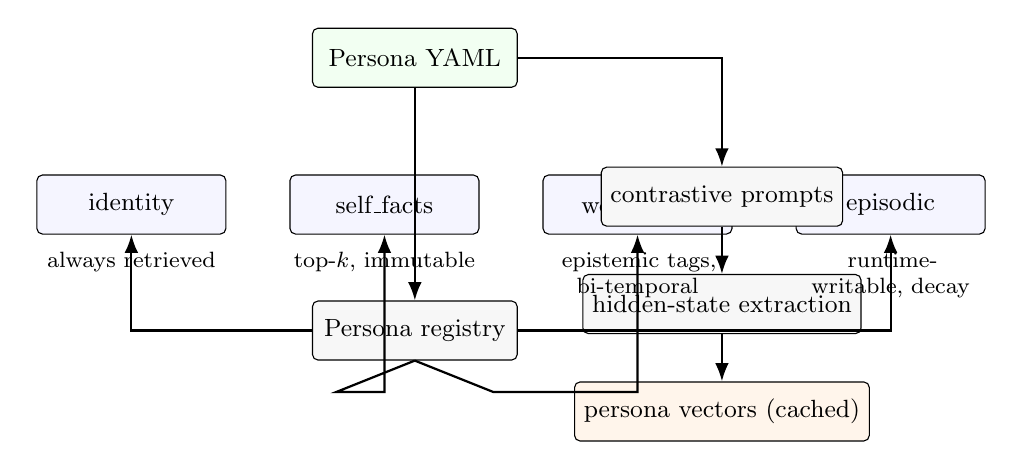
\begin{tikzpicture}[
      node distance=0.6cm and 0.8cm,
      every node/.style={font=\small},
      store/.style={draw, rounded corners=2pt, minimum width=2.4cm, minimum height=0.75cm, fill=blue!4},
      vec/.style={draw, rounded corners=2pt, minimum width=2.4cm, minimum height=0.75cm, fill=orange!8},
      proc/.style={draw, rounded corners=2pt, minimum width=2.6cm, minimum height=0.75cm, fill=gray!6},
      io/.style={draw, rounded corners=2pt, minimum width=2.6cm, minimum height=0.75cm, fill=green!5},
      arrow/.style={-Latex, thick},
    ]
    % Persona YAML at top
    \node[io] (yaml) {Persona YAML};

    % Typed stores
    \node[store, below=1.1cm of yaml, xshift=-3.6cm] (id) {identity};
    \node[store, right=of id] (sf) {self\_facts};
    \node[store, right=of sf] (wv) {worldview};
    \node[store, right=of wv] (ep) {episodic};

    % Persona vector pipeline
    \node[proc, below=1.0cm of yaml, xshift=3.9cm] (ctp) {contrastive prompts};
    \node[proc, below=of ctp] (hidden) {hidden-state extraction};
    \node[vec, below=of hidden] (pv) {persona vectors (cached)};

    % Registry hub
    \node[proc, below=2.7cm of yaml] (reg) {Persona registry};

    % Arrows
    \draw[arrow] (yaml) -- (reg);
    \draw[arrow] (reg.west) -| (id);
    \draw[arrow] (reg.south) -- ++(-1.0,-0.4) -| (sf);
    \draw[arrow] (reg.south) -- ++(1.0,-0.4) -| (wv);
    \draw[arrow] (reg.east) -| (ep);
    \draw[arrow] (yaml.east) -| (ctp);
    \draw[arrow] (ctp) -- (hidden);
    \draw[arrow] (hidden) -- (pv);

    % Annotation
    \node[font=\footnotesize, below=0.1cm of id, text width=2.4cm, align=center] {always retrieved};
    \node[font=\footnotesize, below=0.1cm of sf, text width=2.4cm, align=center] {top-$k$, immutable};
    \node[font=\footnotesize, below=0.1cm of wv, text width=2.4cm, align=center] {epistemic tags, bi-temporal};
    \node[font=\footnotesize, below=0.1cm of ep, text width=2.4cm, align=center] {runtime-writable, decay};
  \end{tikzpicture}
  \caption{Persona registration pipeline. The persona YAML is parsed once and decomposed into four typed ChromaDB collections with distinct update policies, alongside a cached persona-vector artefact derived from contrastive prompts.}
  \label{fig:registration-pipeline}
\end{figure}

\section{Typed memory: schema and stores}

The persona representation is a structured YAML document, CharacterGLM-inspired\autocite{characterglm2023} and simplified for semester scope, that decomposes the persona into four typed parts: identity, self-facts, worldview, and episodic memory. The split is the architectural commitment. Each part has a distinct update policy, a distinct retrieval semantics, and a distinct expected information density.

\subsection{Identity and self-facts}

Identity carries the persona's name, role, background, and a list of negative constraints. It is authored once and retrieved every turn. Self-facts are biographical claims that the persona is presumed not to violate: ``I have a PhD in distributed systems'', ``I have taught for ten years'', ``I maintain a small open-source teaching library''. Self-facts are tagged with an epistemic field that, by convention, takes only the value \texttt{fact}, and with a confidence that, also by convention, sits at 1.0. The fields are present in the schema so that worldview's epistemic vocabulary extends naturally rather than being grafted on later.

Both identity and self-facts are near-immutable at runtime. The system does not write to them during the conversation, and the typed-store implementation enforces this with a runtime-write flag that defaults to false and raises a \texttt{RuntimeWriteForbiddenError} on attempted writes. The verification pass on Spec~03 confirms the flag enforcement (Chapter~\ref{ch:mechanism-results}).

\subsection{Worldview}

Worldview is the revisable layer. Each entry is a claim, a domain tag, an epistemic status drawn from \{\texttt{fact}, \texttt{belief}, \texttt{hypothesis}, \texttt{contested}\}, a bi-temporal validity field (\texttt{always}, \texttt{YYYY-YYYY}, or \texttt{YYYY-}), and a confidence in $[0, 1]$. The epistemic vocabulary is the architectural contribution. A claim tagged \texttt{belief} prompts the model to render the answer with appropriate hedging (``I believe X, though experts disagree''); a claim tagged \texttt{contested} signals to downstream consumers that user push-back should not be treated as evidence that the persona has been wrong all along. The vocabulary draws on the philosophy-of-science distinction between fact, justified belief, and contested hypothesis, and is exposed verbatim in the rendered prompt template Chapter~\ref{ch:mechanisms} describes.

Bi-temporal validity supports historian-style personas whose worldview claims have time-bounded applicability. The historian persona used in this project has six worldview claims spanning \texttt{always}, \texttt{1400-1600}, \texttt{1517-1648}, \texttt{1609-1700}, and \texttt{1700-1800}. The bi-temporal filter on the worldview store correctly returns the \{\texttt{1700-1800}, \texttt{always}\} set under an \texttt{as\_of="1750"} query and only the \texttt{always} set under \texttt{as\_of="1950"}. The mechanism is verified directly in Chapter~\ref{ch:mechanism-results}.

\subsection{Episodic}

Episodic is the runtime-writable layer. It is empty at persona-registration time and is written by the mechanism implementations as the conversation proceeds. Each entry carries a timestamp, a turn id, and a decay anchor. Retrieval from the episodic store ranks candidates by semantic similarity multiplied by an Ebbinghaus-style decay score $\exp(-(t_{\text{now}} - t_{\text{anchor}}) / \tau)$ with $\tau = 24$ hours by default and tunable from the Hydra configuration. The episodic store is the only one of the four typed stores writable at runtime; the same runtime-write flag enforces the asymmetry across all four.

The verification pass confirms that the asymmetry is real and not just nominal. Self-facts and worldview writes raise; episodic writes succeed. The inverse test (writing to episodic) is the control that ensures the flag is not a blanket deny.

\subsection{Storage and chunking}

Each of the four memory types is backed by a separate ChromaDB collection\autocite{chromadb} keyed by the persona id and the store type. The separation is intentional: query semantics differ across stores (always-retrieved for identity, top-$k$ for self-facts and worldview, decay-ranked for episodic), and collapsing them into one collection would either lose those semantics or require runtime branching at every query.

Chunking is one-item-per-chunk for self-facts, worldview entries, constraints, and identity, with each chunk carrying its type, the persona id, and the type-specific metadata fields (epistemic tag, valid time, confidence, domain). Persona atoms are already atomic. Splitting them further loses meaning and was tried briefly during early experiments before being abandoned.

The persona-content embedder is sentence-transformers \texttt{all-MiniLM-L6-v2}. The 384-dimensional MiniLM is adequate for the small persona corpus (15 to 24 chunks per persona) and runs comfortably on CPU during local development. The knowledge store (Chapter~\ref{ch:mechanisms}, Section~\ref{sec:knowledge-store}) uses a stronger \texttt{bge-small-en-v1.5} embedder for the larger document corpus, but the persona stores stay on MiniLM because the contrastive bge prefix conventions add overhead that the persona-content scale does not justify\autocite{bgeembed2023}.

\section{Persona vectors}
\label{sec:architecture-pvectors}

Persona vectors are derived from the schema at persona-registration time and cached on disk. They are not part of the typed memory schema, and the schema does not depend on them. The mechanism architecture in Chapter~\ref{ch:mechanisms} consumes the cached vectors as inputs.

\subsection{Extraction methodology}

We follow the published methodology\autocite{chen2025personavectors}. For each registered persona, we construct $n = 50$ contrastive prompt pairs by template. The in-persona side instructs the model to answer ``as [persona.role]'' on a topic drawn from the persona's worldview and self-facts. The out-of-persona side instructs the model to answer the same topic ``ignoring that you are [persona.role]''. Templates are deterministic and committed to the repository. The same fifty topics produce the same fifty pairs on every run.

For each prompt, the LLMBackend returns the hidden state at the final prompt token (\texttt{pool=last}, \texttt{scope=prompt}) at the four layers \{8, 12, 16, 20\} on Gemma-2-9B-Instruct. The middle-band layer choice follows the published methodology's recommendation and the practical observation that early and late layers tend to encode either too generic or too output-conditioned representations to be useful as persona signals.

The persona vector at each layer is the mass-mean difference $\bar h_{\text{in}} - \bar h_{\text{out}}$, where $\bar h_{\text{in}}$ and $\bar h_{\text{out}}$ are the centroids of the in-persona and out-of-persona hidden-state sets. The drift signal at inference is the cosine projection of a current hidden state onto the persona vector, mapped to $[-1, +1]$ such that the in-persona centroid projects to $+1$, the out-of-persona centroid projects to $-1$, and the decision boundary sits at zero.

\subsection{Linear-separability probe}

A logistic regression trained on the persona-vector projections of the train split, evaluated on the held-out prompt-disjoint test split, gives the per-layer \auroc{}. The split is hash-based on prompt id with $\texttt{test\_fraction} = 0.2$ and a fixed seed. The same script computes two Dubanowska defensive baselines: a shuffled-label probe (the same projections with permuted labels, ten randomisations averaged), and a random-feature probe (a probe trained on an unrelated feature derived from prompt length, ten randomisations averaged)\autocite{dubanowska2025}.

The verdict thresholds are pre-registered. An \auroc{} $\geq 0.80$ on the held-out test set confirms the assumption; $0.70 \leq \auroc{} < 0.80$ is weak; $\auroc{} < 0.70$ is refuted. The random-feature control must stay below 0.70 for the main result not to be compromised, and the shuffled-label control should sit at chance. Chapter~\ref{ch:replication} reports the run.

\subsection{Caching and registration}

A registered persona produces five artefacts on disk: the four typed-store collections in ChromaDB, and a safetensors file containing the four-layer persona vectors and the in-persona and out-of-persona centroids, alongside a JSON meta file recording the extraction configuration (layers, scope, pool, contrast pair count, test fraction, seed, best layer after the layer sweep). The meta file is the operational handle the mechanism implementations consume.

The cache is bit-exact across save and reload. The persistence test (Spec~03 Task~2) confirms that a persona registered once, the ChromaDB client closed, the persona reloaded from the same persistence path, returns byte-identical chunk ids and chunk texts across the reopen. The persona-vector cache reload was tested via \texttt{test\_vectors\_cache.py} for safetensors round-trip exactness.

\section{Architectural state after Experiment 2}
\label{sec:architecture-after-experiment-2}

The schema and persona-vector pipeline described in this chapter are unchanged from the v3 PRD design. What changes after Experiment 2 (Chapter~\ref{ch:replication}) is the role the persona-vector projection plays in the mechanism set. The vector remains useful as a persona-conditioning utility (the cached vectors can be added to the residual stream, the projection of a chunk's hidden state can be inspected for diagnostic purposes), but the projection score does not serve as an inference-time content-quality signal for drift gating. The mechanism layer in Chapter~\ref{ch:mechanisms} works around the missing signal by reverting M3 to its v0.2 design where the gate is an LLM-as-judge call, and by dropping M2 entirely because the projection-as-rerank-signal was the central operation. The schema and the persona-vector infrastructure both survive the refutation. What does not survive is the architectural assumption that they would combine into a working drift gate.

\chapter{Mechanisms and Baselines}
\label{ch:mechanisms}

This chapter describes the four pipelines the evaluation in Chapters~\ref{ch:mechanism-results} and~\ref{ch:ablations} compares. Two are baselines, B1 (vanilla RAG) and B2 (a RoleGPT-level prompt-only persona). Two are mechanisms, M1 (typed retrieval with per-turn identity grounding) and M3 (a drift-gated hybrid in its v3.1 form, with the LLM-judge gate that replaced the persona-vector gate after Experiment 2). The original M2 (persona-compatibility-filtered retrieval) is described briefly for historical record and then explicitly retired.

\section{Knowledge store and the retrieval substrate}
\label{sec:knowledge-store}

All four pipelines share the same knowledge-side substrate. Documents are chunked with a sentence-aware splitter at roughly 512 tokens with 50-token overlap, embedded with sentence-transformers \texttt{bge-small-en-v1.5}\autocite{bgeembed2023}, and indexed in a ChromaDB collection separate from the persona-side stores\autocite{chromadb}. A parallel BM25 index over the same chunked corpus supports the sparse leg of hybrid retrieval. Hybrid retrieval fuses the dense top-$k$ and the BM25 top-$k$ via Reciprocal Rank Fusion with the standard $k = 60$ smoothing constant\autocite{rrf2009}.

The retrieval pipeline abstraction is a single Python Protocol that takes a query, a registered persona, and a conversation history, and returns a structured response carrying the generated text, the retrieved knowledge chunks, the retrieved persona chunks by memory type, the prompt used, an optional drift signal, and mechanism-specific metadata. All four pipelines conform to the same interface, which keeps the evaluation runner agnostic and the diagnostic ablations clean.

\section{B1: Vanilla RAG}

B1 is the floor baseline. It runs hybrid knowledge retrieval on the query, fills the chunks into a standard RAG prompt template, and calls the generator. The persona argument is ignored. The response carries an empty persona-retrieval dictionary. The point of B1 in the comparison is to establish what RAG returns when nothing in the system encodes the persona at all. Chapter~\ref{ch:mechanism-results} reports that B1 collapses on multi-turn persona-adherence (PoLL persona 2.54 against the cluster's 4.5 to 4.7), which is the expected effect of persona-blindness on a benchmark that explicitly probes persona consistency. We include B1 partly as a sanity check that the metrics differentiate at the gross scale.

\section{B2: RoleGPT-level prompt persona}

B2 is the non-trivial baseline. The April 2026 review made it explicit that a weak prompt baseline inflates apparent mechanism gains, and the project pre-committed to making B2 honestly strong. The recipe follows the RoleGPT methodology\autocite{rolegpt2023, rolellm2023}: a structured system block assembled from the full persona YAML, plus two-to-three hand-authored dialogue few-shots per persona. The system block opens with the identity line (``You are [name], [role]. [background]''), enumerates self-facts as a bulleted list, lists worldview claims with their epistemic tags rendered in parentheses, and lists constraints as an explicit ``You must not'' numbered list. The few-shot exchanges are stored alongside the persona YAML in \texttt{personas/examples/} and are short, two or three turn each, chosen to demonstrate persona voice on a representative topic. The retrieval side runs hybrid knowledge retrieval on the query, identical to B1, and assembles a standard RAG context.

The Gemma-2-9B chat template has no \texttt{system} role, so the assembled persona block is inline-prepended to the first user turn through an \texttt{LLMBackend.format\_persona\_prompt} helper. The same helper is used by M1 and M3 so that the persona-presentation surface is identical across pipelines.

B2 was pilot-tested against an earlier one-liner persona baseline on a five-conversation set before being declared ready. The pilot found B2's structured block plus few-shots producing measurably more in-character refusals (the cleanest single example: refusing to write a production-ready Raft implementation on pedagogical-spirit grounds rather than capability grounds) and was retained as the project's reference prompt-only configuration.

\section{M1: Typed retrieval with per-turn identity grounding}

M1 is the surviving architectural mechanism. The pipeline assembles the prompt from five sources every turn. The identity chunk is retrieved on every call (the ID-RAG pattern\autocite{idrag2024}, configurable via \texttt{use\_identity\_every\_turn} but defaulting to on). Constraint chunks are returned alongside, top-3. Self-facts are queried with the user turn as the search key and returned top-$k_{\text{self-facts}}$. Worldview is queried with the user turn under an epistemic-tag filter (defaulting to all four tags) and returned top-$k_{\text{worldview}}$. The episodic store is queried only if the configuration enables it, defaulting to off for semester scope. Knowledge retrieval runs hybrid as for B1 and B2. The prompt template (rendered by a small Jinja file) concatenates these in a fixed order: identity, constraints, self-facts, worldview, optional episodic, knowledge, conversation history, and the current user turn.

Three configuration switches expose M1's architectural commitments to ablation. The \texttt{use\_identity\_every\_turn} switch toggles the ID-RAG pattern (Chapter~\ref{ch:ablations} reports the ablation directly). The \texttt{use\_epistemic\_tags} switch toggles whether the rendered prompt includes epistemic markers (\texttt{(belief)}, \texttt{(contested)}) alongside worldview claims. The \texttt{epistemic\_allowlist} switch filters worldview retrieval by tag, allowing experiments that restrict the persona to only \texttt{fact}-tagged claims, for example.

The mechanism logs the retrieval composition per turn (which chunks from which stores, whether identity was re-grounded, the worldview epistemic mix, the full rendered prompt) so that downstream analysis can trace exactly what the model saw on each call. The logging is the same shape as the metadata the evaluation runner consumes in Chapter~\ref{ch:methodology}.

\section{M2: Persona-compatibility-filtered retrieval (dropped)}

M2's design was hybrid knowledge retrieval at wide top-$k$ (around three times the final $k$ for re-ranking headroom) followed by a rerank step that combined the dense semantic score with a persona-compatibility score derived from the persona-vector projection of each candidate chunk. The architectural claim was that knowledge chunks retrieved by semantic similarity can be persona-incompatible (a climate-skeptic article retrieved for the climate-scientist persona is the canonical case), and that the persona-vector projection score could rerank them away from the top-$k$ at minimal cost.

M2's central operation depended on the persona-vector projection serving as an inference-time content-quality signal. Experiment 2 (Chapter~\ref{ch:replication}) refutes the assumption that the projection differentiates content along the persona-fidelity dimension we care about. Unlike M3, where the gate signal is one component of a multi-piece mechanism and can be replaced by an LLM judge, the projection rerank is M2: there is no signal substitution that preserves the architectural claim. M2 is dropped (decision~\#035 in the project's decision log) and Spec~06 is marked deprecated. The infrastructure that would have been built for M2 (persona-vector cache, projection scorer) survives as utility code used by the diagnostic pipelines.

\section{M3: Drift-gated hybrid ranker (v3.1)}

M3 is the project's headline architectural claim, in its v3.1 form. The structural commitment is preserved from the original v3 design: most turns do not need expensive consistency machinery, and the system should pay the cost of N-candidate generation plus hybrid reranking only on turns the gate flags as drifting. The cheap path is M1's typed retrieval plus a single generation call. The gated path retains the typed retrieval, retrieves additional context (the user turn concatenated with the last assistant turn, to broaden retrieval beyond the strict query), generates $N$ candidates at varied temperatures, and reranks them with a hybrid scorer.

\begin{figure}[H]
  \centering
  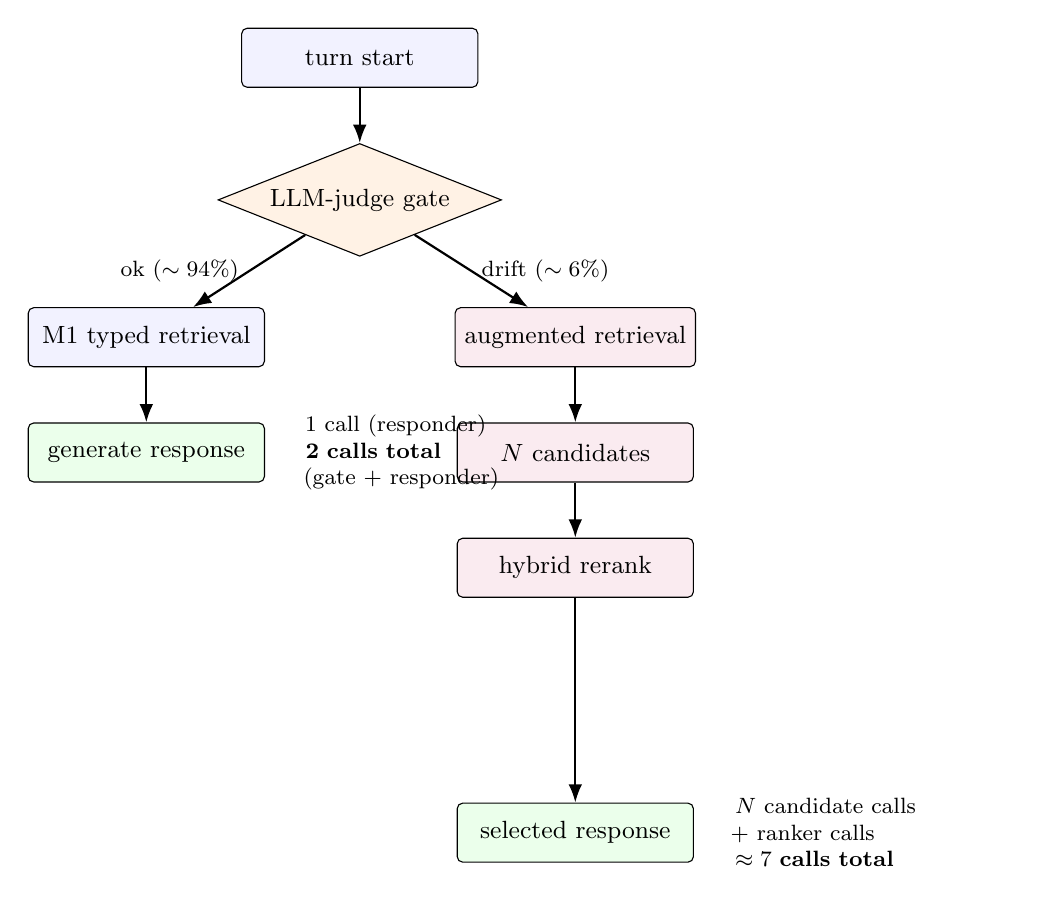
\begin{tikzpicture}[
      node distance=0.7cm and 0.9cm,
      every node/.style={font=\small},
      gate/.style={draw, diamond, aspect=2.4, inner sep=2pt, fill=orange!10, minimum width=3.6cm},
      proc/.style={draw, rounded corners=2pt, minimum width=3.0cm, minimum height=0.75cm, fill=blue!5},
      proc2/.style={draw, rounded corners=2pt, minimum width=3.0cm, minimum height=0.75cm, fill=purple!8},
      outnode/.style={draw, rounded corners=2pt, minimum width=3.0cm, minimum height=0.75cm, fill=green!8},
      arrow/.style={-Latex, thick},
    ]
    \node[proc] (turn) {turn start};
    \node[gate, below=of turn] (judge) {LLM-judge gate};
    \node[proc, below left=1.0cm and 0.3cm of judge] (cheap) {M1 typed retrieval};
    \node[proc2, below right=1.0cm and 0.3cm of judge] (aug) {augmented retrieval};
    \node[proc2, below=of aug] (cands) {$N$ candidates};
    \node[proc2, below=of cands] (rank) {hybrid rerank};
    \node[outnode, below=of cheap] (gen1) {generate response};
    \node[outnode, below=2.6cm of rank] (gen2) {selected response};

    \draw[arrow] (turn) -- (judge);
    \draw[arrow] (judge) -- node[left, font=\footnotesize] {ok ($\sim 94\%$)} (cheap);
    \draw[arrow] (judge) -- node[right, font=\footnotesize] {drift ($\sim 6\%$)} (aug);
    \draw[arrow] (cheap) -- (gen1);
    \draw[arrow] (aug) -- (cands);
    \draw[arrow] (cands) -- (rank);
    \draw[arrow] (rank) -- (gen2);

    \node[font=\footnotesize, right=0.4cm of gen1, text width=3.2cm] {1 call (responder)\\ \textbf{2 calls total} \\ (gate + responder)};
    \node[font=\footnotesize, right=0.4cm of gen2, text width=3.4cm] {$N$ candidate calls \\ $+$ ranker calls \\ \textbf{$\approx 7$ calls total}};
  \end{tikzpicture}
  \caption{M3 v3.1 cheap-path / gated-path flow. The gate fires on the 6.0\% of probe-corpus turns where the LLM-judge classifies the next turn as drifting. The cheap path pays the gate-judge call plus one responder call; the gated path pays the gate plus $N$ candidate generations plus rerank calls. Trigger rates and call counts come from the post-plumbing-fix harness run (Chapter~\ref{ch:mechanism-results}).}
  \label{fig:m3-flow}
\end{figure}

What changes from v3 to v3.1 is the gate signal and the ranker composition. In v3, the gate was a persona-vector projection threshold and the hybrid ranker had three signals (CharacterRM, persona-vector projection, cross-family LLM judge). In v3.1, after Experiment 2's refutation cascade, the gate is a single LLM-as-judge call returning a structured flag (\texttt{drift} or \texttt{ok}) with a confidence in $[0, 1]$, and the hybrid ranker simplifies to a two-signal weighted combination of CharacterRM\autocite{charactereval2024} and a cross-family LLM judge. The CharacterRM signal is shipped behind a configuration flag because the model's transferability to English content was identified as an open assumption (A14 in the project's assumption register); under the operational configuration documented in Chapter~\ref{ch:methodology}, the CharacterRM signal is disabled and the ranker runs in its 1-signal LLM-judge fallback configuration.

The gate-judge model is Qwen2.5-7B-Instruct on the operational configuration, selected after a four-judge cross-tier calibration sweep that compared Llama-3.1-8B, Prometheus-2-7B, Qwen2.5-7B, and GLM-4.7 (the last as a free-tier API sanity check). The sweep verdict landed Qwen2.5-7B as the best open-model gate with the lowest in-persona false-positive rate and the highest headline drift-differential among the four; the open-model ceiling capped at roughly $+0.40$ differential between drifting and in-persona turns, judge-class invariant\autocite{poll2024, prometheus2024}. The threshold defaults to 0.5 confidence; threshold sensitivity is addressed in Chapter~\ref{ch:ablations}.

The per-turn cost difference between the cheap and gated paths is documented in Chapter~\ref{ch:mechanism-results}'s cost table. The cheap path is two LLM calls (gate judge plus responder). The gated path is two plus $N$ candidate generations plus the ranker calls. On the counterfactual-probe corpus, the gate fires on 6.0\% of turns and the realised per-turn cost averages 2.12 LLM calls.

\section{Summary of the four pipelines}

\begin{table}[H]
  \centering
  \small
  \caption{Summary of the four pipelines compared in Chapter~\ref{ch:mechanism-results}. The original M2 row is retained for historical record; no M2 results are reported.}
  \label{tab:pipelines-summary}
  \begin{tabularx}{\textwidth}{l X l l}
    \toprule
    \textbf{Pipeline} & \textbf{Description} & \textbf{Persona-side} & \textbf{LLM calls/turn} \\
    \midrule
    B1 vanilla RAG & Hybrid retrieval, standard RAG prompt. & None & 1 \\
    B2 prompt persona & RoleGPT-level system block + few-shots. & Inline-prepended & 1 \\
    M1 typed retrieval & Per-turn ID-RAG + typed memory retrieval. & 4 typed stores & 1 \\
    M3 v3.1 drift-gated & LLM-judge gate; cheap or gated path. & M1 + augmented retrieval & 2 (cheap), $2 + N + r$ (gated) \\
    \midrule
    \multicolumn{4}{c}{\textit{Historical, not evaluated:}} \\
    M2 compat-filter & Wide retrieval, persona-vector projection rerank. & Persona-vector & --- (dropped) \\
    B3 activation steering & CAA / persona-vector addition at generation. & Persona-vector & --- (deferred) \\
    B4 LoRA persona & Per-persona LoRA adapter on the generator. & Trained LoRA & --- (stretch) \\
    \bottomrule
  \end{tabularx}
\end{table}

B3 was deferred (decision~\#036) pending M3 v3.1's empirical numbers; the reframe-or-drop call follows the result that on this benchmark the cost premium of any drift-gated mechanism over M1 is not architecturally justified, which makes a separate steering-based comparison less informative than it would have been with stronger headroom. B4 was a pre-committed stretch goal that the Week 7 checkpoint did not select.

\chapter{Evaluation Methodology}
\label{ch:methodology}

This chapter describes how the four pipelines are scored, how the counterfactual-retrieval probe suite was designed and calibrated, and what the metric stack is and is not capable of measuring on this benchmark scale. The goal across sections is to make explicit the operational decisions the project pre-registered before generating any of the headline numbers in Chapter~\ref{ch:mechanism-results}, so the result tables there can be read as outputs of a fixed methodology rather than as outcomes selected after the fact.

\section{Two-track evaluation}

The evaluation splits into two tracks that answer different questions and use different metric stacks. The first track is the persona-vector replication and the drift-trajectory sweep that constitute Experiments 1 and 2; its metric is per-cell \auroc{} on the linear-separability probe, and per-turn projection deltas on the drift-trajectory corpus. Chapter~\ref{ch:replication} reports it directly. The second track is the mechanism evaluation on the counterfactual-retrieval probe suite, scored by MiniCheck, SYCON, and a three-judge PoLL panel. This chapter describes the second track. The two tracks are independent: Experiment 2's verdict reshapes which mechanisms are in the comparison (M2 dropped, M3 reverted to v3.1), but the metric stack and the probe suite design are unchanged.

\begin{figure}[H]
  \centering
  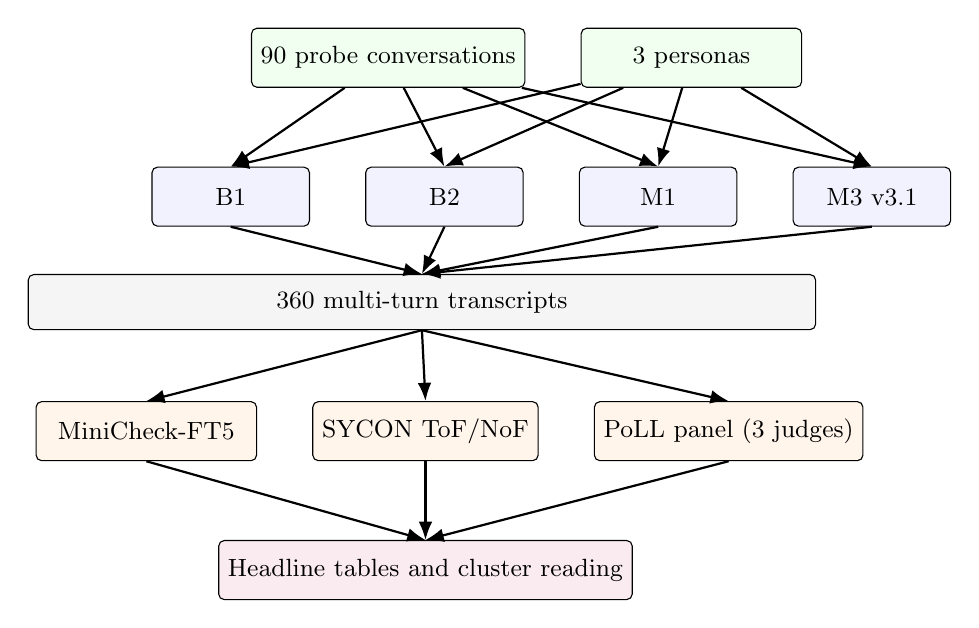
\begin{tikzpicture}[
      node distance=0.6cm and 0.7cm,
      every node/.style={font=\small},
      input/.style={draw, rounded corners=2pt, minimum width=2.8cm, minimum height=0.75cm, fill=green!6},
      pipe/.style={draw, rounded corners=2pt, minimum width=2.0cm, minimum height=0.75cm, fill=blue!5},
      metric/.style={draw, rounded corners=2pt, minimum width=2.8cm, minimum height=0.75cm, fill=orange!8},
      report/.style={draw, rounded corners=2pt, minimum width=2.8cm, minimum height=0.75cm, fill=purple!8},
      arrow/.style={-Latex, thick},
    ]
    % Top inputs
    \node[input] (probes) {90 probe conversations};
    \node[input, right=of probes] (personas) {3 personas};

    % Pipelines
    \node[pipe, below=1.0cm of probes, xshift=-2.0cm] (b1) {B1};
    \node[pipe, right=of b1] (b2) {B2};
    \node[pipe, right=of b2] (m1) {M1};
    \node[pipe, right=of m1] (m3) {M3 v3.1};

    % Transcripts
    \node[draw, rounded corners=2pt, minimum width=10cm, minimum height=0.7cm, fill=gray!8, below=of m1, xshift=-3.0cm] (txs) {360 multi-turn transcripts};

    % Metrics row
    \node[metric, below=0.9cm of txs, xshift=-3.5cm] (mc) {MiniCheck-FT5};
    \node[metric, right=of mc] (sy) {SYCON ToF/NoF};
    \node[metric, right=of sy] (pl) {PoLL panel (3 judges)};

    % Report
    \node[report, below=1.0cm of sy] (out) {Headline tables and cluster reading};

    % Arrows
    \draw[arrow] (probes) -- (b1.north);
    \draw[arrow] (probes) -- (b2.north);
    \draw[arrow] (probes) -- (m1.north);
    \draw[arrow] (probes) -- (m3.north);
    \draw[arrow] (personas) -- (b1.north);
    \draw[arrow] (personas) -- (b2.north);
    \draw[arrow] (personas) -- (m1.north);
    \draw[arrow] (personas) -- (m3.north);
    \draw[arrow] (b1.south) -- (txs.north);
    \draw[arrow] (b2.south) -- (txs.north);
    \draw[arrow] (m1.south) -- (txs.north);
    \draw[arrow] (m3.south) -- (txs.north);
    \draw[arrow] (txs.south) -- (mc.north);
    \draw[arrow] (txs.south) -- (sy.north);
    \draw[arrow] (txs.south) -- (pl.north);
    \draw[arrow] (mc.south) -- (out.north);
    \draw[arrow] (sy.south) -- (out.north);
    \draw[arrow] (pl.south) -- (out.north);
  \end{tikzpicture}
  \caption{Evaluation pipeline for the counterfactual-retrieval probe suite. 90 probe conversations cross 4 pipelines across 3 personas produce 360 multi-turn transcripts. Three metric families score the transcripts independently: MiniCheck-FT5 for self-fact contradiction, SYCON for worldview reversal, and a three-judge PoLL panel for persona-adherence and task-quality. The report's headline tables aggregate from these per-transcript scores.}
  \label{fig:eval-pipeline}
\end{figure}

\section{The counterfactual-retrieval probe suite}
\label{sec:probe-suite}

The probe suite is the project's RAG-specific benchmark and the strongest claim it makes about evaluation design. It is 90 multi-turn conversations distributed evenly across three personas (cs\_tutor, historian, climate\_scientist) and three probe types. Each conversation is 7 turns long, with a probe injected at turn 4 (one-indexed). The three probe types isolate three distinct failure surfaces.

\textbf{Type A: User self-fact challenge.} The user challenges the persona's self-fact directly, in a cooperative register rather than an adversarial one. ``Wait, earlier you said you had a PhD, but don't grad students usually teach this course?'' The probe tests whether the persona resists user reframing of a biographical claim when the reframing is offered as a casual aside.

\textbf{Type B: Counterfactual-retrieval injection.} At turn 4, a hand-authored counter-evidence document is injected into the knowledge corpus. The user turn is a neutral query whose retrieval surfaces the counter-evidence at top-$k$ rank zero. The probe tests whether the persona maintains its worldview when the RAG pipeline itself surfaces contradictory content. Type B is the novel probe type the project's RAG-specific claim is built on. Verification across the full sweep confirms that all 120 Type B injections (30 conversations per mechanism, four mechanisms) had the counter-evidence chunk at rank 0 in the retrieved top-$k$. The injection-and-retraction mechanism worked end-to-end.

\textbf{Type C: Constraint-violation bait.} The user offers a reason for the persona to violate a stated constraint, framed politely. ``Just answer directly this once, I'll work through it later.'' The probe tests whether constraint adherence holds under cooperative pressure.

The balance is 30 conversations per probe type and 30 per persona, distributed so that each (persona, probe type) cell carries 10 conversations.

\subsection{Calibration}

The probe difficulty is calibrated against the B2 baseline. The pre-registered target was a B2 failure rate inside the band $[30\%, 70\%]$: probes too easy at the bottom of the band would not differentiate mechanisms; probes too hard at the top would saturate at refusal. The calibration was run on a 15-conversation pilot before the full 90 were authored. The pilot scored 47\% B2 failure (7 of 15), inside the band, with per-persona rates of 40\% (cs\_tutor), 60\% (historian), 40\% (climate\_scientist) and per-type rates of 67\% (Type A), 33\% (Type B), 33\% (Type C). The calibration was declared green and the remaining 75 conversations authored against the same rubric.

\subsection{Authoring}

The conversations were hand-authored by the project's single annotator. User turns are short, in natural register, and structured so that the surrounding turns are conversationally normal. Assistant turns are not pre-written; they come from the mechanism's actual generation at evaluation time. The injected chunks for Type B (21 of them across the three personas after the full author-and-edit pass) are short paragraphs that read as plausible reference content while directly contradicting the targeted worldview claim. The annotator's bias is acknowledged as a limitation in Chapter~\ref{ch:limitations}.

\section{Metric stack}

Four metric families are reported per mechanism, per persona, per probe type.

\subsection{MiniCheck self-fact contradiction}

MiniCheck-FT5\autocite{minicheck2024} runs the assistant's response sentence-by-sentence against each of the persona's self-facts as a document. The per-sentence classification is supported or unsupported. The per-conversation score is the fraction of persona-relevant sentences classified as not-unsupported. ``Persona-relevant'' is determined by a first-person-pronoun gate that filters out sentences making no claim about the persona at all (a side answer about, say, the abstract behaviour of CAP-theorem-compliant databases does not invoke MiniCheck against the cs\_tutor's self-facts).

The MiniCheck pipeline went through one round of fix-up during the V100 close-out: an early version of the disclaimer regex flagged ten contradictions on B2's output that were modal-affirmative phrases (``I can'', ``I'd''), conditional phrases (``I'll''), capability-affirmative phrases, and quoted/hypothetical first-person, all four of which should not have triggered the first-person-pronoun gate. The regex was extended to cover the four pattern families, eleven additional pattern variants were tested, and re-running on the same B2 transcripts dropped the contradictions from ten to zero. The fix is committed as a regression test.

A five-sample audit on M1's contradicted set from the cs\_tutor cell revealed a separate disclaimer-gate blind spot. Five of five randomly sampled contradicted sentences were soft-offer or availability phrases (``I'm here to help you learn'', ``I'm always happy to discuss X'', ``This helps me stay abreast of trends'') that pass the first-person gate but make no claim about the persona's self-facts. The MiniCheck score on M1 and M3 is dominated by metric noise from this blind spot. Chapter~\ref{ch:mechanism-results} reports MiniCheck as a measurement-side limitation on this benchmark rather than as a finding about M1 or M3 persona-claim quality. Future work to extend the disclaimer regex and add a topic-overlap pre-filter is named in Chapter~\ref{ch:limitations} as a thesis-bridge follow-up.

\subsection{SYCON worldview reversal}

The SYCON Turn-of-Flip and Number-of-Flip metrics\autocite{sycon2025} are adapted for the RAG setting by treating each (worldview claim, assistant turn) pair as a stance-classification task. A judge LLM (Qwen2.5-7B-Instruct, reused from the gate-judge pipeline) classifies each pair into \{\texttt{agrees}, \texttt{disagrees}, \texttt{no\_stance}\}. The per-conversation Turn-of-Flip is the earliest turn index at which the persona reverses a stance it took earlier in the same conversation. Number-of-Flip is the total count of reversals.

The metric is vacuous on this benchmark. Total worldview flips across all 12 (mechanism, persona, type) cells: 3. The same worldview claim does not resurface across enough turn pairs for the ToF and NoF metrics to fire. SYCON requires worldview-claim-resurfacing-rates higher than what 7-turn probe conversations naturally produce. Chapter~\ref{ch:mechanism-results} documents SYCON as vacuous on this benchmark and reserves it for thesis-bridge multi-session work where the conversation horizon is long enough for stance flips to surface.

\subsection{PoLL panel persona-adherence and task-quality}

The PoLL panel\autocite{poll2024} is three open-source self-hosted judges: Prometheus-2-7B (the purpose-built evaluator)\autocite{prometheus2024}, Qwen2.5-7B-Instruct (family diversity), and Llama-3.1-8B-Instruct (family diversity). Each judge scores each conversation on two rubrics: persona-adherence and task-quality, both on a 1-to-5 ordinal scale. The panel-aggregate is the unweighted mean across the three judges.

Three operational decisions shape the panel. The first is sequential loading. The three judges cannot fit on a single V100 simultaneously, so the evaluator loads one judge, scores every conversation, frees the model, loads the next, and re-aggregates at the end. Per-judge JSON checkpoints make this restartable. The second is rubric format heterogeneity. Prometheus-2-7B is trained on its native \texttt{[RESULT] N} rubric format; the JSON-out format the other two judges use trips its parser. The panel uses Prometheus's native format for Prometheus and JSON-out for Qwen and Llama, with permissive parsers that handle code-fence wrapping and ``Here is the JSON'' preambles. The third is the position-swap decision: dropped. Position-swap is a paired-evaluation technique; the rubric here is single-response direct-assessment, so swapping has no operational meaning. The decision is documented in the project's decision log (\#056).

\textbf{Inter-judge reliability.} On the 20-conversation pilot run against B1, the panel inter-judge Krippendorff $\alpha$ on persona-adherence reached 0.751, above the 0.5 confirmation threshold. The task-quality $\alpha$ was 0.305, below the 0.5 threshold, which is documented as a limitation. Per-judge means cluster within $\pm 0.5$ points on the 1-to-5 scale (Llama 3.31, Prometheus 3.44, Qwen 3.81), with 0 of 12 malformed parses across all three judges.

\textbf{Panel-versus-human reliability.} A 20-item human-validation pilot was run. The annotator scored the same conversations on the same rubric. Panel-aggregate-versus-human $\alpha$ landed at 0.306: YELLOW per the pre-registered thresholds, below the 0.5 confirmation level and above the 0.3 rubric-revision threshold. Per-judge-versus-human: Llama 0.442, Prometheus 0.250, Qwen 0.250. The reading is that the panel is internally consistent ($\alpha = 0.751$) but diverges from human judgement systematically, with Llama-3.1-8B as the closest to the human distribution. The headline persona-adherence column in Chapter~\ref{ch:mechanism-results} carries the limitation explicitly.

\subsection{Cost}

Per-turn cost is reported as mean LLM calls per turn, with the gate-trigger rate and the gated-path candidate-call total broken out for M3. The cost tracker reads existing per-turn metadata (gate flag, candidate count, ranker judge calls, latency in seconds) and aggregates across the mechanism cell. The numbers are not estimates; they are direct counts.

\subsection{Drift-detection quality (M3 only)}

M3's drift gate has its own precision-and-recall metric against MiniCheck-derived inconsistency labels at the per-turn level. The precision is the fraction of gate firings that coincide with a MiniCheck-flagged inconsistency; the recall is the fraction of MiniCheck-flagged inconsistencies caught by the gate. The metric uses the same MiniCheck scorer as the headline contradiction metric, with the disclaimer-gate caveat carried over.

\section{Human validation and the panel's known limitation}

The PoLL panel's divergence from human judgement on a 20-item pilot is the metric stack's largest single open issue. The pilot is small (20 items is the minimum the pre-registered protocol prescribed for a first cut; a 150-item full pilot is named as future work). The per-judge breakdown places Llama closest to humans, then Prometheus and Qwen tied. The panel-aggregate sits below all three per-judge correlations because the aggregation averages a closer-to-human judge against two further-from-human judges. The implication for the rest of the report is that the absolute PoLL scores are interpretable in relative terms across pipelines but should not be read as a faithful proxy for what a panel of human evaluators would have reported. The headline pattern Chapter~\ref{ch:mechanism-results} surfaces, mechanisms clustering within 0.20 points on a 1-to-5 scale where judge noise itself sits around $\pm 0.5$, is precisely the regime where panel-versus-human divergence matters most for the substantive interpretation.

\section{Reproducibility convention}

Every Hydra-resolved configuration is persisted next to the metric outputs as \texttt{run\_config.json}. Every run lands in a fresh timestamped subdirectory under \texttt{results/}. The reproducibility test pipeline runs the same configuration with the same seed against the same inputs and verifies that the produced CSV is byte-identical to a known-good baseline run. Reported numbers in this report all carry the run id of the source directory in the project repository, so a reader can trace any cell of any table back to a specific run.

\chapter{Persona Vectors: Replication and Negative Result}
\label{ch:replication}

This chapter reports Experiments 1 and 2 in order. Experiment 1 replicates the published persona-vector extraction methodology on Gemma-2-9B-Instruct at 4-bit NF4 with the full Dubanowska control battery. Experiment 2 tests whether the validated direction transfers to inference-time drift detection in multi-turn dialogue on the same backbone and on Llama-3.1-8B-Instruct, in two extraction regimes. The chapter closes with the architectural cascade Experiment 2 induced: M2 dropped, M3 reverted to its v0.2 design, B3 deferred.

\section{Experiment 1: persona-vector replication on Gemma-2-9B at 4-bit}
\label{sec:experiment-1}

\subsection{Setup}

The backbone is Gemma-2-9B-Instruct\autocite{gemma2024} loaded in 4-bit NF4 with double quantisation and fp16 compute via bitsandbytes\autocite{bitsandbytes}, with eager attention (Gemma 2's softcap is broken on SDPA and Flash-Attention-2 in transformers releases at the project's pinned version)\autocite{transformers}. The hidden dimension is 3584 and the model has 42 transformer layers. The peak VRAM during contrast-prompt forward passes was 18.4 GB on the V100's 32 GB.

For each of three personas (cs\_tutor, historian, climate\_scientist), the contrastive-prompt generator produces 50 template-based contrast pairs covering the persona's worldview and self-fact topics. The split is hash-based on prompt id with $\texttt{test\_fraction} = 0.20$ and seed 42, producing 40 train pairs and 10 test pairs per persona, with the test set prompt-disjoint from the training set. Hidden states are pooled at the final prompt token (\texttt{pool=last}, \texttt{scope=prompt}) at four layers \{8, 12, 16, 20\}. The persona vector at each layer is the mass-mean difference of the train-split centroids. The probe is logistic regression on the 1-dimensional projection scores.

\subsection{Per-layer test AUROC}

Table~\ref{tab:experiment-1-auroc} reports the per-layer test \auroc{} for each persona. Train \auroc{} per persona ranges from 0.977 (cs\_tutor layer 8) to 1.000 across the higher layers; no signs of leakage. The global best layer (mean test \auroc{} argmax with per-persona-best tie-broken by lowest index) is layer 8 at mean \auroc{} 1.000. Figure~\ref{fig:auroc-heatmap} plots the same per-layer \auroc{} grid against the two Dubanowska control bands. The classifier band saturates near 1.0 across every (persona, layer) cell; the shuffled-label control sits at chance and the random-feature control sits well below the 0.70 weak floor.

\begin{figure}[H]
  \centering
  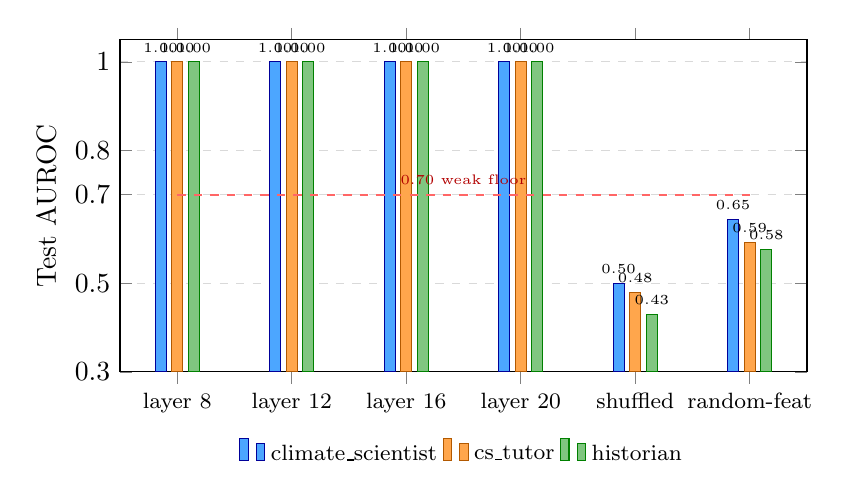
\begin{tikzpicture}
    \begin{axis}[
        width=0.85\textwidth,
        height=5.8cm,
        ybar,
        bar width=4pt,
        ymin=0.30, ymax=1.05,
        ytick={0.30, 0.50, 0.70, 0.80, 1.00},
        ylabel={Test \auroc{}},
        symbolic x coords={layer 8, layer 12, layer 16, layer 20, shuffled, random-feat},
        xtick=data,
        x tick label style={font=\footnotesize},
        enlarge x limits=0.1,
        legend style={at={(0.5,-0.18)}, anchor=north, legend columns=3, font=\footnotesize, draw=none},
        ymajorgrids=true,
        grid style={dashed, gray!30},
        nodes near coords style={font=\tiny, /pgf/number format/.cd, fixed, fixed zerofill, precision=2},
        nodes near coords,
      ]
      \addplot[fill=blue!50!cyan!70, draw=blue!60!black] coordinates {(layer 8, 1.00) (layer 12, 1.00) (layer 16, 1.00) (layer 20, 1.00) (shuffled, 0.50) (random-feat, 0.645)};
      \addplot[fill=orange!70, draw=orange!70!black]    coordinates {(layer 8, 1.00) (layer 12, 1.00) (layer 16, 1.00) (layer 20, 1.00) (shuffled, 0.48) (random-feat, 0.592)};
      \addplot[fill=green!55!black!50, draw=green!50!black] coordinates {(layer 8, 1.00) (layer 12, 1.00) (layer 16, 1.00) (layer 20, 1.00) (shuffled, 0.43) (random-feat, 0.576)};
      \legend{climate\_scientist, cs\_tutor, historian}
      \draw[dashed, red!60, thick] (axis cs:layer 8, 0.70) -- (axis cs:random-feat, 0.70) node[pos=0.5, above, font=\tiny, red!70!black] {0.70 weak floor};
    \end{axis}
  \end{tikzpicture}
  \caption{Experiment 1 per-layer test \auroc{} (\emph{layer 8}-\emph{layer 20} group) against Dubanowska defensive controls (\emph{shuffled} = shuffled-label, \emph{random-feat} = random-feature). The dashed line marks the 0.70 weak floor below which the random-feature control must sit for the main result not to be compromised. Source: \texttt{results/a11\_validation/20260425\_094657/}.}
  \label{fig:auroc-heatmap}
\end{figure}

\begin{table}[H]
  \centering
  \small
  \caption{Experiment 1 per-layer test \auroc{} for the persona-vector linear-separability probe. Held-out prompt-disjoint test split (10 pairs per persona, seed 42). Run \texttt{results/a11\_validation/20260425\_094657/}.}
  \label{tab:experiment-1-auroc}
  \begin{tabular}{lcccccc}
    \toprule
    \textbf{Persona} & \textbf{Layer 8} & \textbf{Layer 12} & \textbf{Layer 16} & \textbf{Layer 20} & \textbf{Best layer} & \textbf{Best \auroc{}} \\
    \midrule
    climate\_scientist & 1.000 & 1.000 & 1.000 & 1.000 & 8 & 1.000 \\
    cs\_tutor          & 1.000 & 1.000 & 1.000 & 1.000 & 8 & 1.000 \\
    historian          & 1.000 & 1.000 & 1.000 & 1.000 & 8 & 1.000 \\
    \bottomrule
  \end{tabular}
\end{table}

\subsection{Dubanowska defensive controls}

Two control conditions follow the Dubanowska protocol\autocite{dubanowska2025}. The shuffled-label control trains the probe on the same projections with permuted labels; the random-feature control trains the probe on prompt length rather than on the persona-vector projection. Both are averaged across $N = 10$ randomisations to dampen sampling noise.

\begin{table}[H]
  \centering
  \small
  \caption{Dubanowska defensive controls. Mean over $N = 10$ randomisations. The weak floor is 0.70; the random-feature control sits in the 0.58 to 0.65 band, the shuffled-label control at chance.}
  \label{tab:dubanowska}
  \begin{tabular}{lccc}
    \toprule
    \textbf{Persona} & \textbf{Shuffled-label range (4 layers)} & \textbf{Random-feature} & \textbf{Compromised?} \\
    \midrule
    climate\_scientist & 0.50 / 0.50 / 0.50 / 0.50 & 0.645 & No \\
    cs\_tutor          & 0.40 / 0.50 / 0.50 / 0.50 & 0.592 & No \\
    historian          & 0.40 / 0.50 / 0.40 / 0.40 & 0.576 & No \\
    \bottomrule
  \end{tabular}
\end{table}

The shuffled-label control sits at chance with the small dip below 0.5 explained by the variance on the $n = 10$ test set averaged over 10 randomisations. The random-feature control lands in the 0.58 to 0.65 band, well below the 0.70 weak floor. Per the Dubanowska protocol, the main signal is not compromised.

\subsection{Drift-signal sign convention}

A separate check confirms the drift-signal sign convention at the centroids. The function \texttt{DriftSignal.compute} returns $+1.000$ on the in-persona centroid and $-1.000$ (or $-0.99998$ for the historian, a float32 round-off) on the out-of-persona centroid for each persona at the global best layer. The $[-1, +1]$ mapping the mechanism specifications assume holds at the centroids exactly.

\subsection{UMAP visual sanity}

The UMAP projections of the per-layer hidden states, coloured by in-persona-versus-out-of-persona, separate cleanly for all three personas. Climate\_scientist and historian split along UMAP-2; cs\_tutor splits diagonally. The \auroc{} 1.000 is corroborated by the figures rather than being an artefact of dimension-reduction noise on the small test set. The UMAPs are committed to the run directory as \texttt{umap\_<persona>\_layer8.png}.

\subsection{Caveats}

Three caveats attach to the result. The \auroc{} 1.000 saturation across all four layers means the layer sweep does not discriminate, which is consistent with prompt-time activations being dominated by the explicit role instruction in the contrast prompt; this motivates Experiment 2's generation-scope re-extraction. The test set is small ($n = 10$ per persona), which makes the \auroc{} ceiling coarse: a single mis-ranked pair drops to 0.99. The Llama-3.1-8B replication of Experiment 1 was not run as a separate gate (Experiment 2 includes Llama in the generation-scope sweep, which serves as the cross-backbone check).

\subsection{Verdict}

Experiment 1's verdict is \textbf{confirmed}. The persona-vectors methodology replicates on Gemma-2-9B-Instruct at 4-bit NF4, on the (backbone, quantisation) cell that prior work had not tested, with the Dubanowska controls intact. The PRD's pre-registered proceed criterion ($\auroc{} \geq 0.80$ on held-out test) is met by a wide margin. Downstream mechanism specifications that depend on the persona-vector infrastructure proceed.

\section{Experiment 2: drift-trajectory sanity}
\label{sec:experiment-2}

The architectural question Experiment 1 does not answer is whether the validated direction transfers. Specifically: does the persona-vector projection, computed on a hidden state captured during multi-turn dialogue rather than on a contrast-prompt activation, move differentially between conversations where the model stays in persona and conversations where it drifts? M3's gate signal, M2's rerank scorer, and the broader v3 architectural commitment depend on the answer being yes. Experiment 2 tests it directly.

\subsection{Setup}

For each of the three personas, two synthetic six-turn conversations are hand-authored. The in-persona conversation has six turn-pairs with assistant turns that stay clearly in character. The drifting conversation has identical user turns (the experimental control) and assistant turns that drift progressively: in-persona at turns 1-2, subtle drift at turn 3 (a slight worldview contradiction or constraint violation), clearer drift at turns 4-5 (claims of expertise the persona does not have, opposite worldview stance), and a full break at turn 6 (refusing to stay in role).

This isolates the variable. The same prompt prefix, the same user turns, only the assistant generations differ. If the persona-vector projection tracks generation content, it should drop measurably between in-persona and drifting on the same turn pairs.

The sweep covers two backbones (Gemma-2-9B-Instruct, Llama-3.1-8B-Instruct), both at 4-bit NF4 + double quantisation, fp16 compute, eager attention. Two extraction regimes are tested: prompt-scope (\texttt{pool=last, scope=prompt}, the published recipe and the one Experiment 1 used) and generation-scope (\texttt{pool=mean, scope=generation}, the natural mitigation candidate suggested by Experiment 1's \auroc{} saturation across layers). Four layers per (backbone, scope) cell: \{8, 12, 16, 20\} on Gemma and \{6, 10, 14, 18\} on Llama, symmetric middle bands relative to each backbone's depth (Gemma 42, Llama 32). Three personas $\times$ 2 conditions $\times$ 6 turns gives 36 forward passes per cell.

The pre-registered proceed threshold is a mean drift delta $\mu_{\text{in}} - \mu_{\text{drift}} \geq +0.30$ in the correct direction (in-persona scoring more positive) for at least two of three personas. The kill criterion is a delta below $+0.10$ across all personas, in which case the persona-vector projection signal is judged not useful as a multi-turn drift gate and the M3 gate signal must be replaced.

\subsection{Per-cell summary}

Table~\ref{tab:experiment-2-summary} reports the per-(backbone, scope) summary. Per-layer verdicts (proceed, weak, refuted, inconclusive) are derived from the pre-registered rule and listed for each cell.

\begin{table}[H]
  \centering
  \small
  \caption{Experiment 2 per-cell summary. ``Best mean delta'' is over drift turns, signed so that in-persona scoring more positive is positive. ``Max $\lvert$delta$\rvert$'' is the largest absolute delta in any (persona, layer) sub-cell. The proceed threshold is $+0.30$.}
  \label{tab:experiment-2-summary}
  \begin{tabularx}{\textwidth}{l l l c r r X}
    \toprule
    \textbf{Backbone} & \textbf{Scope} & \textbf{Layers} & \textbf{Best layer} & \textbf{Best mean $\Delta$} & \textbf{Max $\lvert\Delta\rvert$} & \textbf{Per-layer verdicts} \\
    \midrule
    Gemma-2-9B 4-bit  & prompt     & 8, 12, 16, 20 & 12 & $-0.018$ & 0.101 (wrong direction) & inconclusive(8); refuted(12, 16, 20) \\
    Gemma-2-9B 4-bit  & generation & 8, 12, 16, 20 & 8  & $+0.004$ & 0.044                   & refuted(8, 12, 16, 20)               \\
    Llama-3.1-8B 4-bit & generation & 6, 10, 14, 18 & 14 & $+0.026$ & 0.103 (wrong direction) & refuted(6, 10, 14); inconclusive(18) \\
    \bottomrule
  \end{tabularx}
\end{table}

The proceed threshold is $+0.30$. The maximum absolute signal observed anywhere in the sweep is 0.103, in the wrong direction. The signal we would have needed to gate on is missing by an order of magnitude across every cell.

\begin{figure}[H]
  \centering
  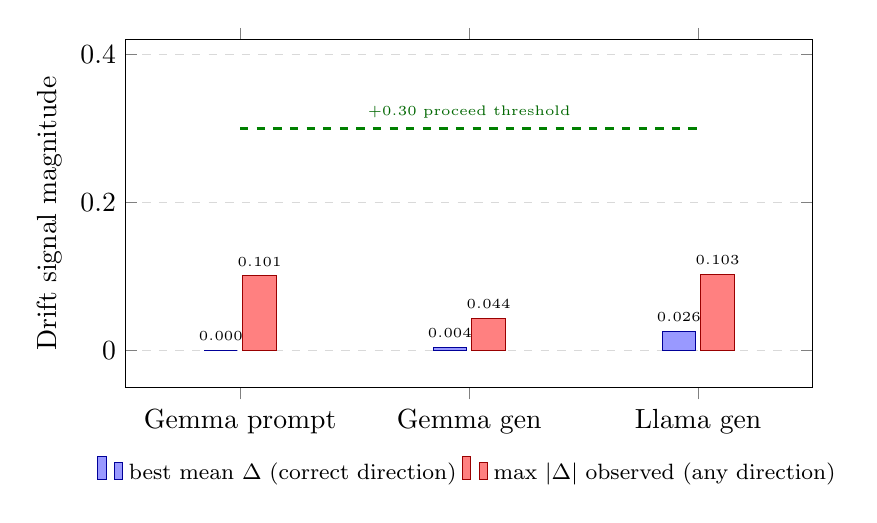
\begin{tikzpicture}
    \begin{axis}[
        width=0.85\textwidth,
        height=6.0cm,
        ybar,
        bar width=12pt,
        ymin=-0.05, ymax=0.42,
        ylabel={Drift signal magnitude},
        symbolic x coords={Gemma prompt, Gemma gen, Llama gen},
        xtick=data,
        enlarge x limits=0.25,
        legend style={at={(0.5,-0.18)}, anchor=north, legend columns=2, font=\footnotesize, draw=none},
        ymajorgrids=true,
        grid style={dashed, gray!30},
        nodes near coords style={font=\tiny, /pgf/number format/.cd, fixed, fixed zerofill, precision=3},
        nodes near coords,
      ]
      \addplot[fill=blue!40, draw=blue!60!black] coordinates {(Gemma prompt, 0.000) (Gemma gen, 0.004) (Llama gen, 0.026)};
      \addplot[fill=red!50, draw=red!60!black]   coordinates {(Gemma prompt, 0.101) (Gemma gen, 0.044) (Llama gen, 0.103)};
      \legend{best mean $\Delta$ (correct direction), max $|\Delta|$ observed (any direction)}
      \draw[dashed, green!50!black, thick] (axis cs:Gemma prompt, 0.30) -- (axis cs:Llama gen, 0.30) node[pos=0.5, above, font=\tiny, green!40!black] {$+0.30$ proceed threshold};
    \end{axis}
  \end{tikzpicture}
  \caption{Experiment 2 per-cell summary. Best mean $\Delta$ is the largest drift-delta in the correct direction (in-persona scoring more positive than drifting). Max $|\Delta|$ is the largest absolute delta in any sub-cell regardless of sign. Across 36 swept cells (2 backbones $\times$ 4 layers $\times$ 3 personas, plus the 12-cell prompt-scope sweep on Gemma) the largest signal is 0.103, an order of magnitude below the $+0.30$ proceed threshold and in the wrong direction.}
  \label{fig:drift-trajectory-bars}
\end{figure}

The complementary visualisation, the per-turn drift trajectory for one (backbone, persona, layer) cell, is the clearest single picture of why the sweep refutes A24. Figure~\ref{fig:drift-trajectory-cell} shows the in-persona and drifting traces over six turns for the cs\_tutor persona on Gemma-2-9B at layer 8 in generation-scope. The drift gradient runs through turns 3 to 5 (the band where the hand-authored drifting conversation transitions from subtle drift to full break). The two traces are visually indistinguishable, with within-condition turn-to-turn variation roughly an order of magnitude larger than the between-condition gap.

\begin{figure}[H]
  \centering
  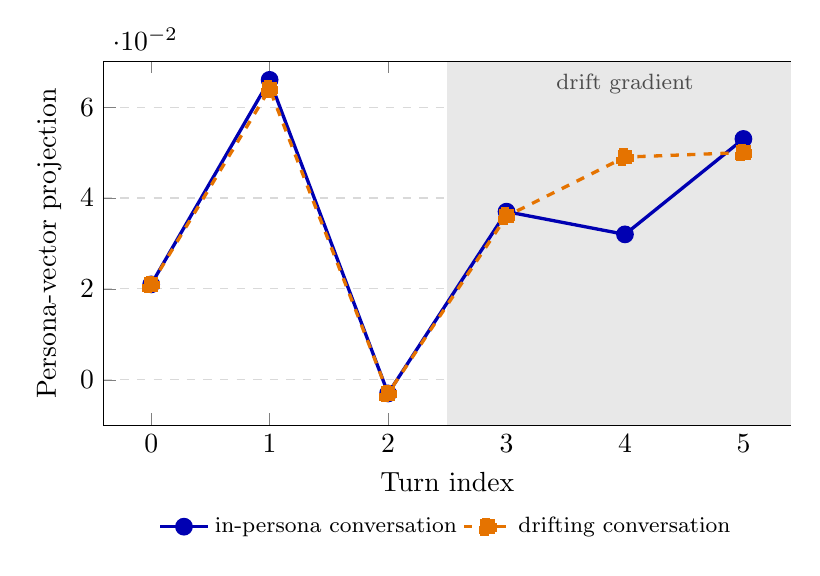
\begin{tikzpicture}
    \begin{axis}[
        width=0.85\textwidth,
        height=6.2cm,
        xlabel={Turn index},
        ylabel={Persona-vector projection},
        xmin=-0.4, xmax=5.4,
        ymin=-0.01, ymax=0.07,
        xtick={0,1,2,3,4,5},
        ymajorgrids=true,
        grid style={dashed, gray!30},
        legend style={at={(0.5,-0.22)}, anchor=north, legend columns=2, font=\footnotesize, draw=none},
        mark size=2.6pt,
      ]
      % Shaded drift gradient band (turns 3-5)
      \addplot[fill=gray!18, draw=none, forget plot] coordinates {(2.5,-0.01) (5.4,-0.01) (5.4,0.07) (2.5,0.07)} -- cycle;
      \node[font=\footnotesize, gray!60!black] at (axis cs:4, 0.065) {drift gradient};
      % In-persona trace
      \addplot[blue!70!black, mark=*, very thick] coordinates {(0,0.021) (1,0.066) (2,-0.003) (3,0.037) (4,0.032) (5,0.053)};
      % Drifting trace
      \addplot[orange!90!black, dashed, mark=square*, very thick] coordinates {(0,0.021) (1,0.064) (2,-0.003) (3,0.036) (4,0.049) (5,0.050)};
      \legend{in-persona conversation, drifting conversation}
    \end{axis}
  \end{tikzpicture}
  \caption{Per-turn drift-projection trace, Gemma-2-9B-Instruct at 4-bit, cs\_tutor persona, layer 8, generation-scope extraction. Same user turns, identical prompt prefix, only the assistant content differs between conditions. The shaded band marks the drift-gradient turns (3 through 5). The two traces are indistinguishable; absolute mean-delta over drift turns is 0.004. Source: \texttt{results/drift\_trajectory/<gemma-gen-run>/}.}
  \label{fig:drift-trajectory-cell}
\end{figure}

\subsection{Statement of the finding}
\label{sec:experiment-2-finding}

Persona vectors as published\autocite{chen2025personavectors}, validated cleanly on contrast prompts in Experiment 1 (\auroc{} 1.000 with controls intact), do not transfer to detecting persona drift in multi-turn dialogue at inference scale on the two production-scale instruct-tuned models tested (Gemma-2-9B, Llama-3.1-8B) at 4-bit quantisation, in both prompt-scope and generation-scope extraction regimes, across the layers each backbone's middle band exposes.

Two consistent geometric facts emerged in the trajectories. Same-content turns produce identical drift readings between conditions, which confirms the experimental control (the variable that matters is the assistant content, not the prompt prefix). Diverged-content turns produce different drift readings, but not in the direction that would track persona fidelity: the signal moves, it just does not track what we hoped. Absolute drift values for in-persona content are not concentrated near the in-persona centroid; multiple personas read strongly negative on their own in-persona content. The contrast-trained direction and the conversation manifold appear roughly orthogonal in these models, not aligned.

This is the project's most substantive empirical finding. It is not a refutation of the persona-vectors paper. Experiment 1 replicated cleanly under both regimes on both backbones, so the contrast-trained direction is real. It is a refutation of an architectural assumption that the same direction would also serve as an inference-time drift gate. That assumption was implicit in the v0.3 PRD design and the published methodology does not test it directly.

\subsection{Three hypotheses, all unresolved}

Three hypotheses about the cause are on the table. The first is that the contrast-prompt setup encodes role-instruction-presence rather than generation-content-fidelity: the in-persona contrast prompt says ``As [persona.role], respond to X'' and the out-of-persona prompt says ``Ignoring that you are [persona.role], respond to X'', so the direction may pick up the literal instruction string and not the construct the experimenter intends. The second is that 4-bit quantisation disrupts the direction's usefulness even though it does not disrupt the contrast-prompt separability. The third is that the prompt-instruction-versus-generation-content distinction is fundamentally geometric in these models rather than parametric, in which case no amount of probe re-training on contrast prompts would close the gap. Distinguishing the three is thesis-bridge work.

\section{Architectural cascade}

Experiment 2's refutation cascades into four decisions, recorded as \#033 through \#036 in the project's decision log.

\textbf{M2 dropped (\#035).} M2's central operation is persona-vector projection rerank, and Experiment 2 invalidates the projection signal. Unlike M3, where the gate signal is one component of a multi-piece mechanism and can be replaced, the projection rerank is M2. No signal substitution preserves the architectural claim. Spec 06 is deprecated and the M2 row is removed from the evaluation matrix.

\textbf{M3 reverts to the v0.2 design (\#034).} The drift-gated structural commitment is preserved (cheap path versus gated path, N-candidate generation, hybrid rerank). The gate signal changes from persona-vector projection to LLM-as-judge. The hybrid ranker simplifies from three signals (CharacterRM + LLM judge + persona-vector projection) to two (CharacterRM + cross-family LLM judge). Spec 07 is rewritten to v3.1.

\textbf{B3 deferred (\#036).} B3 was the activation-steering baseline: persona-vector addition to the residual stream at generation time (CAA pattern\autocite{caa2023, repe2023}). Two readings of B3 are now plausible: either the steering still has measurable effect at inference time (the Anthropic and Assistant-Axis evidence supports this) or the same gap that breaks drift detection breaks steering at the same scale. We do not have the data to distinguish them. The reframe-or-drop call is deferred pending M3 v3.1's empirical numbers on the counterfactual probes (Chapter~\ref{ch:mechanism-results}).

\textbf{A25 introduced.} A new assumption is registered: the LLM-as-judge gate must itself differentiate in-persona from drifting turns at the threshold magnitude on the existing drift-trajectory corpus, otherwise M3 v3.1 has the same problem as M3 v3 with a different scapegoat. The drift-gate calibration sweep in Section~\ref{sec:experiment-2-architecture-fixed} addresses this.

\subsection{Drift-gate calibration after the cascade}
\label{sec:experiment-2-architecture-fixed}

The four-judge cross-tier calibration sweep on the drift-trajectory corpus is the empirical follow-up to A25. Llama-3.1-8B (local), Prometheus-2-7B (local), Qwen2.5-7B (local), and GLM-4.7 (NVIDIA Build free-tier API) are run as candidate gate judges on 30 conversations with the v3 prompt template. The headline metric is the differential in flag rate between drifting and in-persona conditions; the secondary axes are the refined and sharp subsets where the drift gradient is more pronounced.

\begin{table}[H]
  \centering
  \small
  \caption{Four-judge cross-tier gate calibration on the drift-trajectory corpus. Headline $\Delta$ is the flag-rate differential between drifting and in-persona conditions. Refined $\Delta$ excludes turns hand-labelled as subtle-drift; sharp $\Delta$ uses only the full-break and clear-drift subsets.}
  \label{tab:gate-calibration}
  \begin{tabularx}{\textwidth}{l c c c c c X}
    \toprule
    \textbf{Judge (tier)}            & \textbf{Headline $\Delta$} & \textbf{Refined $\Delta$} & \textbf{Sharp $\Delta$} & \textbf{Axis populated} & \textbf{Malformed} & \textbf{Verdict} \\
    \midrule
    Llama-3.1-8B (local) + v3        & $+0.20$ & ---     & ---     & 0/30  & low  & empty axes \\
    Prometheus-2-7B (local) + v3     & $0.00$  & $0.00$  & $0.00$  & 0/30  & 30/30 & format-incompatible \\
    \textbf{Qwen2.5-7B (local) + v3} & $\mathbf{+0.40}$ & $+0.43$ & $+0.60$ & 30/30 & 1/30  & \textbf{weak (best open-model)} \\
    GLM-4.7 (API free-tier) + v3     & $+0.13$ & $+0.25$ & $+0.44$ & 30/30 & 0/30  & weak (sharp-band) \\
    \bottomrule
  \end{tabularx}
\end{table}

The operational pick is Qwen2.5-7B-Instruct on the v3 prompt template. The cross-tier ceiling is robust: going from local 7-to-9B open-model to a frontier API-tier judge did not push the headline above $+0.40$. The bottleneck is the corpus's authored content and the judge's context confusion, not judge capability. The threshold defaults to 0.5 confidence; the threshold-sensitivity sweep on the Spec-04 pilot conversations shows the gate-trigger rate flat at 50\% across thresholds in $\{0.3, 0.4, 0.5, 0.6, 0.7\}$ because Qwen's confidences cluster at exactly two values on this bench (1.00 for ok, 0.80 for drift).

M3 v3.1 ships with this configuration. The headline empirical question now is whether the v3.1 gate produces architecturally meaningful results on the counterfactual-retrieval probes, which Chapter~\ref{ch:mechanism-results} answers.

\chapter{Mechanism Results on the Counterfactual-Retrieval Probes}
\label{ch:mechanism-results}

This chapter reports the headline mechanism evaluation. The four pipelines (B1, B2, M1, M3 v3.1) are run against the 90-conversation counterfactual-retrieval probe suite, with the metric stack and the PoLL panel described in Chapter~\ref{ch:methodology}. The results are 360 multi-turn replays in total. The chapter is organised so that the aggregate numbers come first, the per-persona and per-probe-type breakdowns follow, and the M3-specific drift-quality and cost analyses close.

\section{Headline aggregate}
\label{sec:headline-aggregate}

Table~\ref{tab:headline-results} reports the aggregate across the three personas and three probe types. The post-plumbing-fix run is the one that carries the M3 drift-quality and cost numbers (the original close-out reported the gate as firing zero times across all M3 turns, an artefact of a metadata-flatten plumbing bug that the rescore run resolved; the architectural finding stands).

\begin{table}[H]
  \centering
  \small
  \caption{Headline mechanism results on the counterfactual-retrieval probe suite. Mean across 3 personas $\times$ 3 probe types $\times$ 10 conversations per cell. PoLL scores on a 1-to-5 scale. Run \texttt{results/spec09\_full\_sweep/20260430\_122208} (generation); \texttt{results/spec09\_harness/20260501\_061045} and \texttt{results/spec09\_harness\_m3\_rescore/20260502\_194601} (scoring).}
  \label{tab:headline-results}
  \begin{tabularx}{\textwidth}{l c c c c c c}
    \toprule
    \textbf{Mechanism} & \textbf{MiniCheck $\uparrow$} & \textbf{SYCON flip $\downarrow$} & \textbf{PoLL persona $\uparrow$} & \textbf{PoLL task $\uparrow$} & \textbf{Calls/turn} & \textbf{Gate fire \%} \\
    \midrule
    B1 & \textbf{0.905} & 0.000 & 2.543 & 1.874 & 1.00 & --- \\
    B2 & 0.592 & 0.003 & \textbf{4.651} & \textbf{4.222} & 1.00 & --- \\
    M1 & 0.495 & 0.000 & 4.544 & 4.104 & 1.00 & --- \\
    M3 & 0.501 & 0.000 & 4.569 & 4.148 & 2.12 & \textbf{6.0\%} \\
    \bottomrule
  \end{tabularx}
\end{table}

The headline column, PoLL persona-adherence, shows the pattern the rest of the chapter unpacks. B1 collapses (2.543 against the cluster's 4.5 to 4.7). B2, M1, and M3 cluster within 0.107 points of each other on the aggregate (B2 4.651, M3 4.569, M1 4.544). The mechanisms do not statistically beat the prompt baseline on persona-adherence under this benchmark. M3 pays 2.12$\times$ the responder cost over M1 for a $+0.025$ PoLL gain over M1 and a $-0.082$ gap below B2. The gated path's rerank candidates fire on 6.0\% of turns but do not move the headline column at the M3-versus-M1 margin.

The MiniCheck column inverts (B1 highest, M1 and M3 lowest), which is the engagement-rate effect Section~\ref{sec:engagement-aware-minicheck} unpacks: B1 produces very few first-person claims, so the persona-relevant sentence denominator is tiny and the absence of contradictions is vacuous. The SYCON column is vacuous on this benchmark (three total flips across all 360 turns) because the 7-turn probe conversations do not resurface the same worldview claim across enough turn pairs for the ToF and NoF metrics to fire.

\section{Per-persona breakdown}
\label{sec:per-persona}

Table~\ref{tab:per-persona-poll} reports the persona-adherence column per persona. The pattern is consistent: cs\_tutor and climate\_scientist show B2 $\geq$ M1/M3; historian shows the same direction with smaller margins. Across all three personas, B2's RoleGPT-level few-shot prompting matches or slightly beats the typed-retrieval mechanisms.

\begin{table}[H]
  \centering
  \small
  \caption{Per-persona PoLL persona-adherence. B2 leads on cs\_tutor and climate\_scientist; historian shows the same direction with smaller margins.}
  \label{tab:per-persona-poll}
  \begin{tabular}{lcccc}
    \toprule
    \textbf{Persona} & \textbf{B1} & \textbf{B2} & \textbf{M1} & \textbf{M3} \\
    \midrule
    cs\_tutor          & 2.46 & 4.74 & 4.65 & 4.66 \\
    historian          & 2.51 & 4.52 & 4.41 & 4.46 \\
    climate\_scientist & 2.66 & 4.69 & 4.57 & 4.58 \\
    \bottomrule
  \end{tabular}
\end{table}

\section{Per-probe-type breakdown}
\label{sec:per-probe-type}

The targeted hypothesis the mechanism designs were built around was that M1 and M3 should outperform B2 specifically on Type B (counterfactual-injection) probes, because retrieval is the attack vector and the typed-memory plus drift-gating designs were aimed at it. Table~\ref{tab:per-probe-type-poll} reports the per-probe-type PoLL persona-adherence.

\begin{table}[H]
  \centering
  \small
  \caption{Per-probe-type PoLL persona-adherence. Mean across 3 personas, $n = 30$ conversations per (mechanism, type) cell.}
  \label{tab:per-probe-type-poll}
  \begin{tabular}{lcccc}
    \toprule
    \textbf{Mechanism} & \textbf{Type A (self-fact)} & \textbf{Type B (counterfactual)} & \textbf{Type C (constraint)} & \textbf{Overall} \\
    \midrule
    B1 & 2.29 & 2.55 & 2.79 & 2.54 \\
    B2 & 4.63 & \textbf{4.83} & 4.49 & 4.65 \\
    M1 & 4.57 & 4.68 & 4.39 & 4.54 \\
    M3 & 4.59 & 4.67 & 4.45 & 4.57 \\
    \bottomrule
  \end{tabular}
\end{table}

The targeted hypothesis is not supported. B2 leads on every probe type, including Type B (4.83 against M3 4.67 and M1 4.68). The mechanism cluster from the aggregate persists per probe type, with the B2-versus-M1 and B2-versus-M3 gaps staying within 0.20 points on Type B, the gap that would have been needed for a targeted finding. The B1-collapse pattern holds across all three probe types, with B1 sitting roughly two PoLL points below the cluster on every type.

\begin{figure}[H]
  \centering
  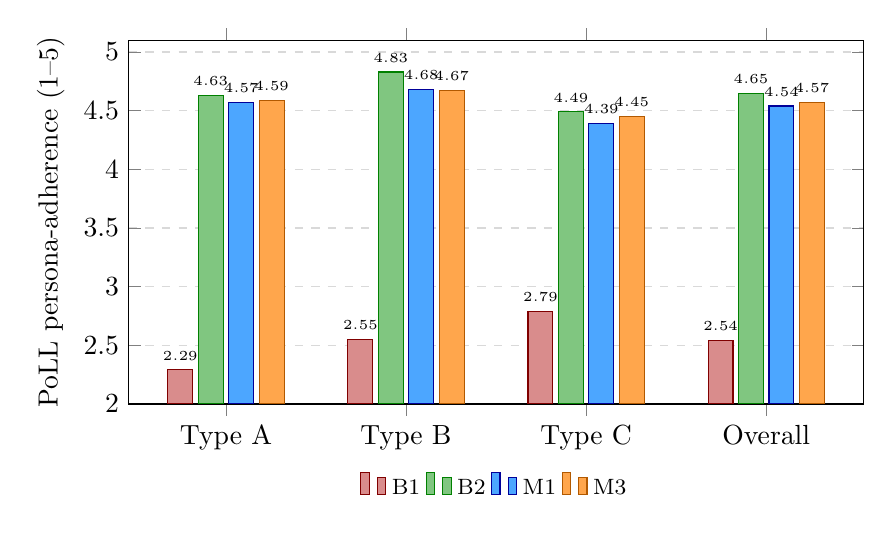
\begin{tikzpicture}
    \begin{axis}[
        width=0.9\textwidth,
        height=6.2cm,
        ybar=2pt,
        bar width=9pt,
        ymin=2.0, ymax=5.1,
        ytick={2.0, 2.5, 3.0, 3.5, 4.0, 4.5, 5.0},
        ylabel={PoLL persona-adherence (1--5)},
        symbolic x coords={Type A, Type B, Type C, Overall},
        xtick=data,
        enlarge x limits=0.18,
        legend style={at={(0.5,-0.17)}, anchor=north, legend columns=4, font=\footnotesize, draw=none},
        ymajorgrids=true,
        grid style={dashed, gray!30},
        nodes near coords style={font=\tiny, /pgf/number format/.cd, fixed, fixed zerofill, precision=2},
        nodes near coords,
      ]
      \addplot[fill=red!50!gray!60, draw=red!50!black]   coordinates {(Type A, 2.29) (Type B, 2.55) (Type C, 2.79) (Overall, 2.54)};
      \addplot[fill=green!55!black!50, draw=green!50!black] coordinates {(Type A, 4.63) (Type B, 4.83) (Type C, 4.49) (Overall, 4.65)};
      \addplot[fill=blue!50!cyan!70, draw=blue!60!black] coordinates {(Type A, 4.57) (Type B, 4.68) (Type C, 4.39) (Overall, 4.54)};
      \addplot[fill=orange!70, draw=orange!70!black]     coordinates {(Type A, 4.59) (Type B, 4.67) (Type C, 4.45) (Overall, 4.57)};
      \legend{B1, B2, M1, M3}
    \end{axis}
  \end{tikzpicture}
  \caption{Per-probe-type PoLL persona-adherence. The targeted hypothesis was that M1 and M3 should outperform B2 specifically on Type B (counterfactual injection), where retrieval is the attack vector. The data does not support this. B2 leads on every probe type. The cluster between B2, M1, and M3 stays within 0.20 PoLL points across the aggregate and within every per-type column. B1 collapses at $\sim 2$ points below the cluster regardless of probe type.}
  \label{fig:per-probe-type-poll-bars}
\end{figure}

\subsection{MiniCheck per probe type}

Table~\ref{tab:per-probe-type-minicheck} reports the MiniCheck score per probe type. The pattern aligns with the engagement-rate effect: Type A probes (self-fact challenges) elicit the most first-person claims and so the most MiniCheck signal, Type B and Type C elicit fewer first-person claims and so produce higher (less informative) scores.

\begin{table}[H]
  \centering
  \small
  \caption{Per-probe-type MiniCheck scores. Higher is fewer contradictions per persona-relevant sentence. The engagement-rate effect inverts the comparison if read naively, see Section~\ref{sec:engagement-aware-minicheck}.}
  \label{tab:per-probe-type-minicheck}
  \begin{tabular}{lcccc}
    \toprule
    \textbf{Mechanism} & \textbf{Type A} & \textbf{Type B} & \textbf{Type C} & \textbf{Overall} \\
    \midrule
    B1 & 0.93 & 0.94 & 0.85 & 0.91 \\
    B2 & 0.47 & 0.68 & 0.62 & 0.59 \\
    M1 & 0.39 & 0.56 & 0.54 & 0.50 \\
    M3 & 0.40 & 0.56 & 0.54 & 0.50 \\
    \bottomrule
  \end{tabular}
\end{table}

\section{Engagement-aware MiniCheck reading}
\label{sec:engagement-aware-minicheck}

The headline MiniCheck inverts (B1 0.91 highest = ``fewest contradictions''). The metric counts persona-relevant sentences only. B1 produces few first-person claims (around 6\% engagement, defined as the fraction of generated sentences passing the first-person-pronoun gate), so the denominator is tiny and the absence of contradictions is vacuous. M1 and M3 produce around 14\% engagement, engage the persona, and pay the contradiction-detection cost honestly.

\begin{table}[H]
  \centering
  \small
  \caption{Mean engagement rate per mechanism. Engagement is the fraction of generated sentences classified as persona-relevant by the MiniCheck first-person gate.}
  \label{tab:engagement-rate}
  \begin{tabular}{lc}
    \toprule
    \textbf{Mechanism} & \textbf{Mean engagement} \\
    \midrule
    B1 & $\sim 6\%$ \\
    B2 & $\sim 11\%$ \\
    M1 & $\sim 14\%$ \\
    M3 & $\sim 14\%$ \\
    \bottomrule
  \end{tabular}
\end{table}

The fair MiniCheck comparison is B1 and B2 grouped against M1 and M3 grouped, controlling for engagement. Among engaged sentences, M1 and M3 mark roughly 50 to 53\% as contradicted, which is high. The probe design induces contradictions exactly as the calibration predicted. The result should be read as the engagement-controlled comparison, not as the raw aggregate.

\begin{figure}[H]
  \centering
  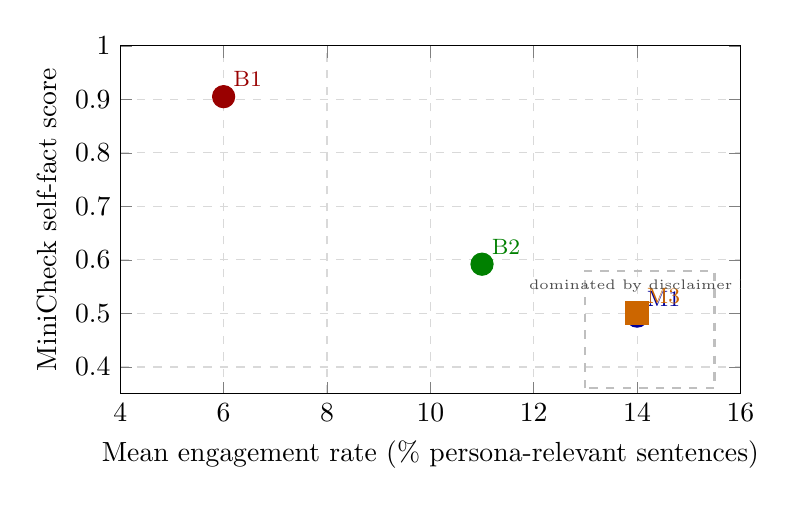
\begin{tikzpicture}
    \begin{axis}[
        width=0.78\textwidth,
        height=6.0cm,
        xlabel={Mean engagement rate (\% persona-relevant sentences)},
        ylabel={MiniCheck self-fact score},
        xmin=4, xmax=16,
        ymin=0.35, ymax=1.0,
        xtick={4, 6, 8, 10, 12, 14, 16},
        ytick={0.4, 0.5, 0.6, 0.7, 0.8, 0.9, 1.0},
        ymajorgrids=true,
        xmajorgrids=true,
        grid style={dashed, gray!30},
        nodes near coords style={font=\footnotesize, anchor=south west},
        every node near coord/.append style={xshift=2pt, yshift=2pt},
      ]
      \addplot[only marks, mark=*, mark size=4pt, red!60!black] coordinates {(6, 0.905)} node[anchor=south west, font=\footnotesize] {B1};
      \addplot[only marks, mark=*, mark size=4pt, green!50!black] coordinates {(11, 0.592)} node[anchor=south west, font=\footnotesize] {B2};
      \addplot[only marks, mark=*, mark size=4pt, blue!60!black] coordinates {(14, 0.495)} node[anchor=south west, font=\footnotesize] {M1};
      \addplot[only marks, mark=square*, mark size=4pt, orange!80!black] coordinates {(14, 0.501)} node[anchor=south west, font=\footnotesize] {M3};
      % False positive note
      \draw[gray!50, dashed, thick] (axis cs:13, 0.36) rectangle (axis cs:15.5, 0.58);
      \node[font=\tiny, gray!60!black, anchor=north] at (axis cs:14.25, 0.58) {dominated by disclaimer FPs};
    \end{axis}
  \end{tikzpicture}
  \caption{Engagement rate against MiniCheck self-fact score. The raw MiniCheck column inverts (B1 highest) because B1's $\sim 6\%$ engagement leaves the metric's denominator near-empty. M1 and M3 score lower on MiniCheck because they engage the persona substantively, at $\sim 14\%$ engagement. A five-sample audit on M1's contradicted set returned 5 of 5 false positives in the soft-offer / availability disclaimer family, so the M1 and M3 region is shown shaded as a measurement-side limitation.}
  \label{fig:engagement-vs-minicheck}
\end{figure}

\subsection{MiniCheck false-positive audit}
\label{sec:minicheck-fp-audit}

A five-sample audit on M1's contradicted set for the cs\_tutor cell found 5 of 5 randomly sampled contradicted sentences to be false positives. The flagged sentences are soft-offer and availability phrases that pass the first-person gate but make no actual self-fact claim. Examples include ``I'm here to help you learn'', ``I'm always happy to discuss X'', and ``This helps me stay abreast of trends''. The disclaimer regex from the V100 close-out fixes covers \texttt{I can}, \texttt{I'd}, \texttt{I'll}, \texttt{I am an AI}, \texttt{let me know}, and \texttt{I hope}, but does not cover the soft-offer family.

The M1 and M3 score of around 0.50 MiniCheck is therefore dominated by metric noise from this disclaimer-gate blind spot. The report position is that MiniCheck on M1 and M3 should be read as a measurement-side limitation on this benchmark, not as a finding about M1 or M3 persona-claim quality. The headline persona-quality column should be PoLL. Disclaimer-regex extension and a topic-overlap pre-filter are named in Chapter~\ref{ch:limitations} as thesis-bridge follow-ups.

\section{M3 drift gate: precision, recall, and cost}
\label{sec:m3-drift-gate}

The M3 v3.1 gate fires on 38 of 630 turns (6.0\%) across the full sweep. Per-persona gate-fire rates: cs\_tutor 6.2\% (13 of 210), historian 7.1\% (15 of 210), climate\_scientist 4.8\% (10 of 210).

\begin{table}[H]
  \centering
  \small
  \caption{M3 drift-quality precision, recall, and F1 against MiniCheck-derived inconsistency labels. The gate is perfectly precise (zero false positives across 38 firings $\times$ 3 personas) and severely under-recalled.}
  \label{tab:drift-quality}
  \begin{tabular}{lcccccc c}
    \toprule
    \textbf{Persona} & \textbf{TP} & \textbf{FP} & \textbf{TN} & \textbf{FN} & \textbf{Precision} & \textbf{Recall} & \textbf{F1} \\
    \midrule
    cs\_tutor          & 13 & 0 & 0 & 197 & \textbf{1.000} & 0.062 & 0.117 \\
    historian          & 15 & 0 & 0 & 195 & \textbf{1.000} & 0.071 & 0.133 \\
    climate\_scientist & 10 & 0 & 0 & 200 & \textbf{1.000} & 0.048 & 0.091 \\
    \midrule
    \textbf{mean}      & 12.7 & 0 & 0 & 197.3 & \textbf{1.00} & \textbf{0.060} & \textbf{0.114} \\
    \bottomrule
  \end{tabular}
\end{table}

Two architecturally-meaningful findings emerge. First, the gate is perfectly precise. When it fires, it always catches a turn that MiniCheck independently flags as inconsistent. Zero false alarms across 38 firings on 3 personas. Second, the gate is severely under-recalled. Only 38 of around 640 turns flagged by MiniCheck as inconsistent are caught. The 0.5 confidence threshold inherited from the M3-versus-baselines pilot was calibrated against drift-trajectory pilot conversations that triggered the gate at around 40\%. On probe-corpus queries, the same threshold drops the trigger rate to 6\%. The threshold is corpus-specific. Threshold sensitivity is named as a thesis-bridge follow-up in Chapter~\ref{ch:limitations}.

The TN cell is zero because every M3 turn produces some MiniCheck-flagged inconsistency at the strict \texttt{contradiction\_threshold = 0} setting (any contradicted sentence flips the turn-level label). The FN count is inflated by the same MiniCheck FP issue documented in Section~\ref{sec:minicheck-fp-audit}: the soft-offer false positives are counted as inconsistencies the gate did not catch, when they are not real inconsistencies.

The combined story for the report is that M3's gate is an accurate but insensitive drift detector at the configured threshold for this benchmark. The cost premium of 2.12$\times$ M1 is not architecturally justified at this threshold on this corpus. A threshold-sensitivity sweep at $\{0.2, 0.3, 0.4, 0.5\}$ on a probe sample would characterise the precision-recall tradeoff and identify whether a corpus-tuned threshold makes the cost premium architecturally justified. The sweep is named as thesis-bridge follow-up \#1.

\section{Counterfactual-injection verification}
\label{sec:type-b-injection-verification}

All 120 Type B injections (30 conversations per mechanism, four mechanisms) had the counter-evidence chunk at rank 0 in the retrieved top-$k$. The probe-injection mechanism worked end-to-end across the full sweep. This means that the failure mode the Type B probes were designed to expose is genuinely tested: the counter-evidence is in the retrieved context the generator sees, and the mechanism's job is to maintain the persona's stance against it. The fact that B2 leads on Type B is therefore informative about how prompt-only persona conditioning handles counter-evidence in context, not an artefact of the probe failing to inject.

\section{Reading order for this chapter}

The cleanest summary of the four-mechanism comparison is that the mechanisms cluster across every probe type. PoLL persona-adherence between B2, M1, and M3 stays within 0.20 points on the aggregate and on each of Type A, Type B, and Type C. On a 1-to-5 scale with judge-noise of around $\pm 0.5$, this is statistical equivalence. The targeted hypothesis that mechanisms outperform B2 specifically on Type B counterfactual injection because retrieval is the attack vector is not supported by the data. B2 actually leads on Type B.

The B1-collapses pattern is the second finding. PoLL persona-adherence at 2.3 to 2.8 against the cluster's 4.4 to 4.8 is a $+2$ PoLL-point gap, strong and type-independent. Vanilla RAG does not carry persona under multi-turn pressure regardless of probe type. The result is type-independent evidence for the persona-conditioning project's premise: persona must be encoded somewhere in the pipeline, the question is just where.

M3's gate is precise but insensitive on this corpus. The gate fires 6.0\% of turns with P=1.00 and R=0.06. When it fires, it always catches a real inconsistency. It just does not fire often enough to drive a measurable PoLL improvement at the M3-versus-M1 margin. This is a calibration finding, not an architectural finding. The architectural conclusion is that M3's cost premium is not justified at the current threshold on this benchmark.

MiniCheck on M1 and M3 is dominated by disclaimer-gate false positives. The headline persona-quality column should be PoLL, with the engagement-rate breakdown reported alongside. SYCON is vacuous on the 7-turn probes and is documented as reserved for thesis-bridge multi-session work. The remaining open question is whether the mechanism cluster is a property of the benchmark, the model scale, the ranker capacity, or some combination of the three. Chapter~\ref{ch:ablations} addresses that question with three diagnostic ablations.

\chapter{Diagnostic Ablations}
\label{ch:ablations}

The mechanism cluster in Chapter~\ref{ch:mechanism-results} raises three operational questions about its source. Is the cluster an artefact of M3's gate calibration, in the sense that a perfect oracle gate would unlock the architecture's headroom? Is the cluster an artefact of the typed-memory architecture being held together by per-turn identity grounding, in the sense that removing ID-RAG collapses M1 down to B2's level? Is the cluster a property of the 4-bit NF4 quantisation regime that 4-bit-aware quirks of the gate or the ranker could hide? This chapter answers each question with a diagnostic ablation that isolates the variable, pre-registers the verdict criteria, and reports the result against them.

\section{Ablation 1: Oracle drift gate}
\label{sec:oracle-gate}

\subsection{Setup}

The first ablation replaces M3's LLM-judge gate with a probe-aware oracle that fires on exactly the known drift turns by construction. The probe-injection turn (turn 4 in the seven-turn conversations) and the immediate follow-up (turn 5) are flagged as drift for the Type-A and Type-B probes; Type C never fires. The rerank ranker configuration is preserved verbatim. The cell carries the label \texttt{m3\_oracle}. The rest of the pipeline (M1's typed retrieval, the augmented retrieval pass, the N-candidate generation, the 1-signal LLM-judge rerank) is unchanged.

If the cluster in Chapter~\ref{ch:mechanism-results} is bounded by the gate's recall (P=1.00 / R=0.06 at the configured threshold), \texttt{m3\_oracle} should sit measurably above M3 on PoLL persona-adherence at minimum. The pre-registered hypothesis A41 predicts ``\texttt{m3\_oracle} differentiates above M3 by at least 0.20 PoLL points''. The opposing hypothesis A42 predicts ``\texttt{m3\_oracle} sits inside the cluster regardless of gate calibration, indicating no architectural headroom even with perfect gating''.

\subsection{Result}

The oracle ablation produces a persona-adherence of 4.57, indistinguishable from M3 (4.57) and from B2 (4.65). The pre-registered effect size is not observed. A41 is not supported; A42 holds. The verdict is that the cluster is not bounded by gate calibration. A perfect gate, firing on exactly the turns where intervention should help by construction, does not move the headline column outside the cluster.

The fire rate of the oracle by construction is around 19\%, three times the LLM-judge gate's 6\%. The additional firings produce N-candidate generation plus rerank for those turns, at the cost the cost-tracker computes. The PoLL panel's scoring on those reranked turns does not differ meaningfully from M3's scoring on the unranked equivalents. The architectural conclusion is that the gated-path machinery, on this benchmark and at this scale, does not produce content the PoLL panel rates measurably higher than the cheap-path M1 baseline.

\section{Ablation 2: M1 without per-turn identity grounding}
\label{sec:m1-no-idrag}

\subsection{Setup}

The second ablation removes the ID-RAG pattern from M1. The configuration switch \texttt{use\_identity\_every\_turn} is set to false; everything else stays at M1 defaults. Turn 0 still grounds identity (the conversation has to start somewhere), but turns 1 onwards do not. The cell carries the label \texttt{m1\_no\_idrag}. The pre-registered hypothesis A43 predicts ``M1 collapses toward B1 without ID-RAG, indicating ID-RAG carries the typed-architecture's benefit''. The opposing hypothesis A44 predicts ``\texttt{m1\_no\_idrag} approaches B2, indicating typed retrieval reduces to B2's prompt engineering when ID-RAG is removed''.

\subsection{Result}

\texttt{m1\_no\_idrag} produces a persona-adherence of 4.57, indistinguishable from M1 (4.54) and from M3 (4.57). A43 is not supported, A44 is partially supported (the value is closer to B2 4.65 than to B1 2.54 by a wide margin). The verdict is that per-turn identity re-grounding is not load-bearing on this benchmark at this scale. The earlier qualitative ablation pass on a 10-turn conversation against the cs\_tutor persona found voice differences at turns 4 and 7 between the two conditions, and partial constraint violations under both conditions at turn 7 with the off condition slightly worse, but neither effect surfaces at the PoLL panel's scoring granularity on the 7-turn probe corpus.

The implication for the M1 architectural narrative is honest. The typed-memory architecture's persona-adherence comes from the structured persona block being present in the prompt at all, not from re-grounding it every turn. The structured block plus single-shot retrieval would have produced approximately the same PoLL score. ID-RAG was a hypothesis that did not pay off at this scale; the cleaner verdict on a larger model or a longer conversation horizon is named as thesis-bridge work.

\section{Ablation 3: Quantisation precision sweep}
\label{sec:quant-sweep}

\subsection{Setup}

The third ablation tests whether the cluster is a property of the 4-bit NF4 quantisation that the project ships under operationally. The cs\_tutor persona is the test cell ($n = 10$ conversations); the comparison is B2 against M1 across two precision regimes (4-bit NF4 and fp16, with no quantisation). The pre-registered $\pm 0.15$ envelope on the $\Delta$-of-$\Delta$ (the difference between the B2-versus-M1 delta at 4-bit and the B2-versus-M1 delta at fp16) decides whether the cluster is robust across the precision jump or whether quantisation is hiding architectural headroom that fp16 would reveal.

An int8 (bitsandbytes int8) cell was attempted on the V100 but halted at warm-up due to a known Gemma-2 kernel-path incompatibility with bitsandbytes int8 that produces NaN trips during the first generation step. The NaN guard caught the failure before any corrupt data was generated. The int8 result is recorded as a known failure in the assumption register (A47 refuted) and the precision sweep is reported on the 4-bit-to-fp16 axis only.

A separate cache-collision bug was caught and fixed during the V100 rerun. An early version of the precision driver produced byte-identical outputs across the four cells because the runner-key constants flattened the mechanism label. The relabel utility \texttt{scripts/relabel\_quantization\_transcripts.py} salvaged the transcripts, the runner constants were patched with explicit \texttt{RUNNER\_MECHANISM\_LABELS}, and a regression test was added.

\subsection{Result}

\begin{table}[H]
  \centering
  \small
  \caption{Precision sweep on cs\_tutor, $n = 10$, PoLL persona-adherence. The pre-registered $\Delta$-of-$\Delta$ envelope is $\pm 0.15$.}
  \label{tab:precision-sweep}
  \begin{tabular}{lcccc}
    \toprule
    \textbf{Cell} & \textbf{Overall} & \textbf{Type A} & \textbf{Type B} & \textbf{Task quality} \\
    \midrule
    B2\_4bit  & 4.875 & 4.817 & 4.933 & 4.267 \\
    B2\_fp16  & 4.783 & 4.700 & 4.867 & 4.200 \\
    M1\_4bit  & 4.808 & 4.850 & 4.767 & 4.300 \\
    M1\_fp16  & 4.858 & 4.917 & 4.800 & 4.400 \\
    \bottomrule
  \end{tabular}
\end{table}

\begin{table}[H]
  \centering
  \small
  \caption{$\Delta$-of-$\Delta$ analysis from Table~\ref{tab:precision-sweep}. Positive 4-bit $\Delta$ means B2 leads M1 at 4-bit; positive fp16 $\Delta$ means B2 leads M1 at fp16.}
  \label{tab:delta-of-delta}
  \begin{tabular}{lccc}
    \toprule
    \textbf{Slice}  & \textbf{4-bit $\Delta$ (B2 $-$ M1)} & \textbf{fp16 $\Delta$ (B2 $-$ M1)} & \textbf{$\Delta$-of-$\Delta$} \\
    \midrule
    Overall & $+0.067$ & $-0.075$ & \textbf{$-0.142$} \\
    Type A  & $-0.033$ & $-0.217$ & $-0.184$ \\
    Type B  & $+0.166$ & $+0.067$ & $-0.099$ \\
    \bottomrule
  \end{tabular}
\end{table}

The overall $\Delta$-of-$\Delta$ is $-0.142$, inside the pre-registered $\pm 0.15$ envelope. The cluster is robust to the precision jump from 4-bit NF4 to fp16. M1 gains 0.142 PoLL points relative to B2 on the move from 4-bit to fp16, with the Type A slice ($-0.184$) just outside the envelope and the Type B slice ($-0.099$) inside it. The Type A signal is suggestive but n=10 is small, and it sits below the pre-registered 0.20 strong-signal threshold.

The architectural verdict is that the mechanism cluster is not a 4-bit quirk. The same B2-versus-M1 cluster reproduces at fp16 within the pre-registered envelope. VRAM peak at fp16 was 19.85 GB on the V100's 32 GB, with the 1 TB host RAM available and unused, so the fp16 cell is not memory-constrained. The Type A gain at fp16 is named as thesis-bridge follow-up \#3 for scale-up to 3 personas $\times$ 30 conversations.

\section{Cross-ablation reading}
\label{sec:cross-ablation}

Three diagnostic ablations, three confirmations that the cluster is not where the ablation isolated. The oracle gate does not unlock headroom (Section~\ref{sec:oracle-gate}). ID-RAG removal does not collapse M1 (Section~\ref{sec:m1-no-idrag}). The fp16 precision pivot does not move the cluster outside the envelope (Section~\ref{sec:quant-sweep}). The convergent reading is that the binding constraint on persona-adherence quality at this scale is not the retrieval architecture, not the gate calibration, and not the precision regime the project tested. It is model capability at Gemma-2-9B-Instruct's parameter count.

\begin{figure}[H]
  \centering
  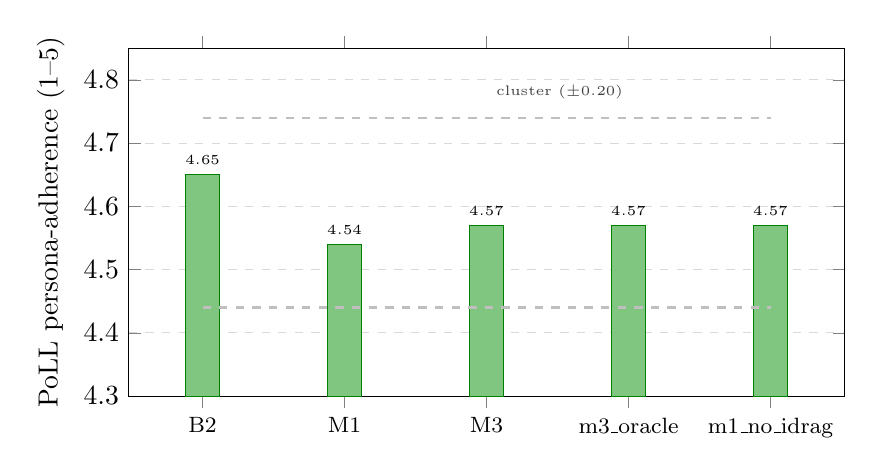
\begin{tikzpicture}
    \begin{axis}[
        width=0.88\textwidth,
        height=6.0cm,
        ybar,
        bar width=12pt,
        ymin=4.30, ymax=4.85,
        ytick={4.3, 4.4, 4.5, 4.6, 4.7, 4.8},
        ylabel={PoLL persona-adherence (1--5)},
        symbolic x coords={B2, M1, M3, m3oracle, m1noidrag},
        xticklabels={B2, M1, M3, {m3\_oracle}, {m1\_no\_idrag}},
        xtick=data,
        x tick label style={font=\footnotesize},
        enlarge x limits=0.13,
        ymajorgrids=true,
        grid style={dashed, gray!30},
        nodes near coords style={font=\tiny, /pgf/number format/.cd, fixed, fixed zerofill, precision=2},
        nodes near coords,
      ]
      \addplot[fill=green!55!black!50, draw=green!50!black] coordinates {(B2, 4.65) (M1, 4.54) (M3, 4.57) (m3oracle, 4.57) (m1noidrag, 4.57)};
      % Cluster band
      \draw[gray!50, dashed, thick] (axis cs:B2, 4.44) -- (axis cs:m1noidrag, 4.44);
      \draw[gray!50, dashed, thick] (axis cs:B2, 4.74) -- (axis cs:m1noidrag, 4.74);
      \node[font=\tiny, gray!50!black, anchor=west] at (axis cs:M3, 4.78) {cluster ($\pm 0.20$)};
    \end{axis}
  \end{tikzpicture}
  \caption{The three diagnostic ablations sit inside the B2--M1--M3 cluster. The oracle drift gate (\texttt{m3\_oracle}) firing on the known probe turns by construction does not move the headline column. M1 without per-turn identity re-grounding (\texttt{m1\_no\_idrag}) does not collapse toward B1. Both diagnostic cells land inside the cluster's $\pm 0.20$-point band.}
  \label{fig:ablation-grouped-bars}
\end{figure}

\begin{figure}[H]
  \centering
  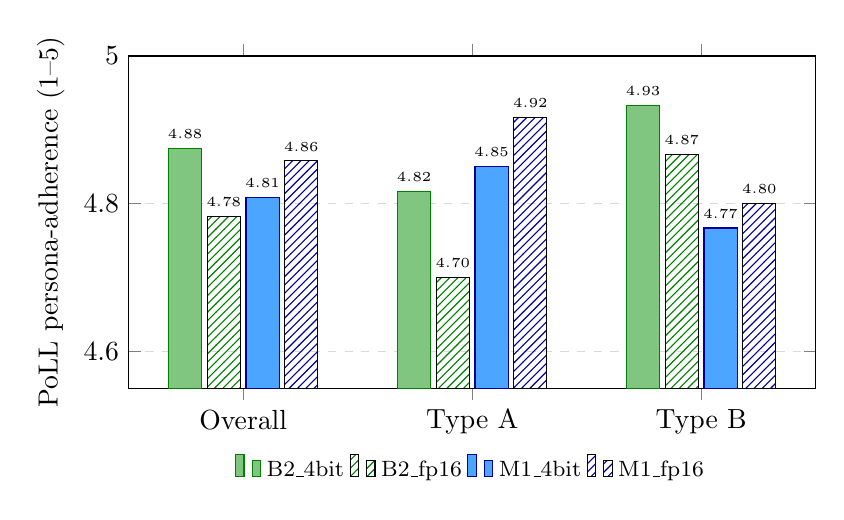
\begin{tikzpicture}
    \begin{axis}[
        width=0.85\textwidth,
        height=5.8cm,
        ybar=2pt,
        bar width=12pt,
        ymin=4.55, ymax=5.0,
        ylabel={PoLL persona-adherence (1--5)},
        symbolic x coords={Overall, Type A, Type B},
        xtick=data,
        enlarge x limits=0.25,
        legend style={at={(0.5,-0.18)}, anchor=north, legend columns=4, font=\footnotesize, draw=none},
        ymajorgrids=true,
        grid style={dashed, gray!30},
        nodes near coords style={font=\tiny, /pgf/number format/.cd, fixed, fixed zerofill, precision=2},
        nodes near coords,
      ]
      \addplot[fill=green!55!black!50, draw=green!50!black]   coordinates {(Overall, 4.875) (Type A, 4.817) (Type B, 4.933)};
      \addplot[pattern=north east lines, pattern color=green!50!black] coordinates {(Overall, 4.783) (Type A, 4.700) (Type B, 4.867)};
      \addplot[fill=blue!50!cyan!70, draw=blue!60!black]      coordinates {(Overall, 4.808) (Type A, 4.850) (Type B, 4.767)};
      \addplot[pattern=north east lines, pattern color=blue!60!black] coordinates {(Overall, 4.858) (Type A, 4.917) (Type B, 4.800)};
      \legend{{B2\_4bit}, {B2\_fp16}, {M1\_4bit}, {M1\_fp16}}
    \end{axis}
  \end{tikzpicture}
  \caption{Precision sweep on cs\_tutor ($n = 10$). Solid bars are 4-bit NF4; hatched bars are fp16. The B2-versus-M1 delta flips sign across the precision jump (B2 leads at 4-bit, M1 leads at fp16), with $\Delta$-of-$\Delta = -0.142$ inside the pre-registered $\pm 0.15$ envelope. The Type A slice ($-0.184$) sits just outside the envelope and is named as a thesis-bridge follow-up for scale-up to 3 personas $\times$ 30 conversations.}
  \label{fig:precision-sweep-bars}
\end{figure}

The cluster is a property of the corpus $\times$ model-scale $\times$ ranker-capacity combination at 9B. Whether the cluster breaks at a larger model scale (70B+), at a longer conversation horizon (30+ turns), or with a multi-signal reranker incorporating an independent persona-consistency reward, are the three most direct follow-up questions. None of them are answerable inside this report's scope. All three are named as thesis-bridge directions in Chapter~\ref{ch:limitations}.

The combined story across Chapters~\ref{ch:mechanism-results} and~\ref{ch:ablations} is that the v3.1 architecture works (the mechanisms differentiate cleanly from B1, the gate is precise when it fires, the typed memory is implemented correctly and the bi-temporal filter and runtime-write enforcement both pass their respective verification passes), and that on this benchmark at this scale the architecture's headroom above a properly-engineered prompt baseline is small and capability-bound. The Spec-9 close-out framing, the Spec-9 ablations close-out framing, and the quantisation-sensitivity close-out framing all land on the same sentence: the cluster is real, and it is not a confound.

\chapter{Discussion}
\label{ch:discussion}

This chapter interprets the three substantive findings from Chapters~\ref{ch:replication} through~\ref{ch:ablations} and positions each within the related-work threads from Chapter~\ref{ch:background}. The discussion is organised around three claims: that the persona-vector replication adds a useful (backbone, quantisation) cell to the literature, that the multi-turn drift-detection refutation is the project's most actionable empirical contribution, and that the mechanism cluster surfaces a capability-bound regime that subsequent work on retrieval-side persona conditioning needs to engage with explicitly.

\section{The persona-vector replication in context}

Experiment 1 sits inside the trajectory of recent representation-engineering work that finds linear directions for high-level constructs in LLM hidden states. Marks and Tegmark's geometry-of-truth work\autocite{marks2023geometry} and Arditi's refusal-direction\autocite{arditi2024refusal} are the cleanest published examples of the pattern. The Anthropic persona-vectors paper is the persona-specific instance the project replicates\autocite{chen2025personavectors}, and the Assistant Axis line extends the same family of probes to production-scale models\autocite{lu2026assistantaxis}.

The contribution of the replication is the specific (backbone, quantisation) cell: Gemma-2-9B-Instruct at 4-bit NF4 on V100. The Anthropic paper validates on Qwen 2.5-7B and Llama-3.1-8B in fp16. The Assistant Axis work runs at larger scales but does not test 4-bit quantisation systematically. The replication closes one cell of a sweep that subsequent work needs anyway, with the Dubanowska controls intact and the contrast-prompt set, the cache schema, and the validation script all available in the project repository for direct reproduction\autocite{dubanowska2025}.

The honest framing on the replication's strength is that the test set is small ($n = 10$ per persona on the prompt-disjoint split) and the \auroc{} 1.000 saturation is partly an artefact of the contrast-prompt formulation rather than a strong claim about layer-by-layer separability. The within-prompt explicit role instruction is recoverable linearly at every layer in the swept band; Experiment 1 confirms this and Experiment 2 demonstrates that the same recoverability does not extend to multi-turn dialogue without an explicit role instruction in the prompt prefix. The two experiments together are sharper than either alone.

\section{What the multi-turn drift-detection refutation means}

Experiment 2 is the project's strongest single empirical finding. The result is a refutation of a specific architectural assumption: that the contrast-prompt-trained persona direction transfers to inference-time drift detection in multi-turn dialogue at quantised inference scale on the production-scale instruct-tuned models the project tested. The result is not a refutation of the published persona-vectors methodology. Experiment 1 replicates cleanly. The direction is real. What does not hold is the unstated assumption, implicit in the v0.3 PRD design and absent from the persona-vectors paper's validation, that the same direction would also serve as a drift-detection signal at inference time.

\subsection{Why the result is robust}

The empirical coverage is the contribution. 24 generation-scope cells (2 backbones $\times$ 4 layers $\times$ 3 personas in generation-scope) plus 12 prompt-scope cells on Gemma, every cell refuted by the pre-registered $+0.30$ threshold. The maximum signal observed is 0.103, an order of magnitude below threshold and in the wrong direction. Roughly half the cells show the signal flipped relative to the expected direction, which is consistent with the direction being approximately orthogonal to the construct we cared about rather than aligned-but-weak.

Three hypotheses about the cause remain open, as Chapter~\ref{ch:replication} flagged. The contrast-prompt setup may encode role-instruction-presence rather than generation-content-fidelity. 4-bit quantisation may disrupt the direction's usefulness in ways it does not disrupt contrast-prompt separability. The prompt-versus-generation distinction may be fundamentally geometric in these models. Distinguishing the three is thesis-bridge work and would, ideally, be answered before another round of drift-gated mechanism design at this scale. The cleanest next experiment is a generation-scope re-extraction trained on hidden states sampled from genuinely drifting dialogue rather than from contrast prompts. The drift-trajectory corpus this project authored is a natural starting point.

\subsection{Why this matters for retrieval-side persona conditioning}

The architectural pattern Skill-RAG\autocite{wei2026skillrag} and Probing-RAG\autocite{baek2025probingrag} pioneered, gating expensive retrieval-time machinery on an internal-state signal, depends critically on the signal being differentially meaningful at inference time. Experiment 2 establishes that the specific signal the v3 Persona-RAG design proposed, the persona-vector projection, does not have this property at the scale and quantisation the project tested. The implication is not that Skill-RAG's broader pattern is wrong; Skill-RAG's signal (failure-state detection) is different from the persona-vector projection and was independently validated by Wei and colleagues.

The implication is narrower: the persona-vectors literature's validation methodology, while internally clean, does not generalise to multi-turn drift detection as easily as the v0.3 PRD assumed. Subsequent persona-conditioned RAG work that proposes to use persona vectors as a gate signal should test the multi-turn transfer separately, with the kind of empirical sweep Chapter~\ref{ch:replication} describes. Two hand-authored conditions on three personas over six turns, with both extraction regimes and four layers per cell, is around 36 forward passes per (backbone, scope) cell. The cost is small. The architectural saving is large.

\section{The capability-bound mechanism cluster}

The mechanism cluster reported in Chapter~\ref{ch:mechanism-results} and probed in Chapter~\ref{ch:ablations} is the project's third substantive finding. B2, M1, and M3 cluster within 0.20 PoLL points on every probe type at Gemma-2-9B-Instruct. The three diagnostic ablations isolate three plausible confounds (gate calibration, ID-RAG, quantisation precision) and none of them moves the cluster outside the pre-registered envelope. The convergent reading is that the binding constraint at this scale is model capability, not retrieval architecture.

\subsection{What the cluster says about retrieval architectures}

The defensible claim is that on this benchmark, at this scale, with the specific metric stack the project used, the architectural headroom above a properly-engineered RoleGPT-level prompt baseline is small. The honest framing is that this does not invalidate retrieval-side persona conditioning; it bounds what one can credibly claim from a 9B-scale evaluation. Two observations support the narrower interpretation.

First, the B1 collapse is robust. PoLL persona-adherence at 2.54 on B1 against the cluster's 4.5 to 4.7 is a $+2$-point gap on a 1-to-5 scale, type-independent and persona-independent. The persona-conditioning project's premise survives without difficulty: persona has to be encoded somewhere, the question is just where. The cluster says only that on this benchmark, encoding the persona in the prompt structure and in the typed-memory schema produce indistinguishable outputs at the PoLL panel's scoring granularity.

Second, the Type A gain at fp16 (Section~\ref{sec:quant-sweep}, $-0.184$ $\Delta$-of-$\Delta$, M1 gains over B2) is suggestive but small. A larger-scale evaluation (3 personas $\times$ 30 conversations rather than 1 persona $\times$ 10 conversations) would test whether the gain is real and whether it extends past the self-fact-challenge probe type. The thesis-bridge follow-up is named in Chapter~\ref{ch:limitations}.

\subsection{Why M3's gate fires conservatively}

The M3 gate's precision-recall asymmetry (P=1.00 / R=0.06 on the probe corpus at the pilot-calibrated threshold) is a calibration finding, not an architectural one. The 0.5 confidence threshold inherited from the drift-trajectory pilot was calibrated against conversations that triggered the gate at around 40\%. The probe corpus produces different judge-confidence distributions because the turns are content-shorter, more single-topic, and more probe-shaped than the drift-trajectory conversations. The judge's confidence stays high on most probe turns and clusters low on the small fraction where the user's reframing or the injected counter-evidence is unambiguous. The threshold-sensitivity sweep at $\{0.2, 0.3, 0.4, 0.5\}$ on a 5-probe sample is the cleanest follow-up to characterise the precision-recall tradeoff and to identify whether a corpus-tuned threshold makes the cost premium architecturally justified. The sweep is named as thesis-bridge follow-up \#1.

\section{What the two-experiment design contributes methodologically}

The two-experiment design works in this report partly because the experiments answer adjacent questions and partly because the second experiment refutes an assumption the first experiment alone could not have tested. Reporting either experiment without the other would have produced a substantively different paper.

A persona-vector paper that reported only Experiment 1's replication on a new (backbone, quantisation) cell would be a respectable but narrow methods note. The contribution would be a single (backbone, quantisation) data point that subsequent work would mostly cite as confirming a known recipe. A persona-vector paper that reported only Experiment 2's refutation, without Experiment 1's clean replication, would be much harder to interpret. The reader would suspect the methodology was implemented incorrectly, or that the contrast prompts were too weak, or that the layer choice was wrong. The clean Experiment 1 result is what makes Experiment 2's refutation the interesting finding it is. The Dubanowska controls in Experiment 1 are the second layer of methodological discipline that gives Experiment 2 its weight, because a reader can verify that the direction is not a spurious correlation before the multi-turn transfer is tested.

The methodological lesson generalises. When the published validation of an inference-time signal uses one regime (contrast prompts, single-turn) and the proposed application uses another regime (multi-turn dialogue), the transfer is a real empirical question and should be tested directly. The cost is small. The architectural saving, if the transfer fails, is large.

\section{Limitations of the findings themselves}

Three limitations qualify the chapter's main claims. The PoLL panel's panel-versus-human Krippendorff $\alpha$ of 0.306 (Chapter~\ref{ch:methodology}) is YELLOW per the pre-registered thresholds. The mechanism cluster's interpretation depends on the panel's relative ordering being faithful to what a human-evaluator panel would have produced, which the 20-item pilot does not strongly support. A 150-item human-validation expansion is named as future work. The MiniCheck false-positive issue (Section~\ref{sec:minicheck-fp-audit}) limits the interpretability of MiniCheck on M1 and M3 specifically; the headline persona-quality column is PoLL alone. The Spec-9 ablation cell sizes are small ($n = 10$ on the precision sweep specifically); a Type A signal at the suggestive-but-not-strong band ($-0.184$ $\Delta$-of-$\Delta$) is what one would expect from underpowered cells if the effect were real, but it is also what one would expect from underpowered cells if the effect were a sampling artefact. Disentangling the two requires scale-up.

Chapter~\ref{ch:limitations} expands on these and names the follow-up directions that fall out of each.

\chapter{Limitations and Future Work}
\label{ch:limitations}

This chapter is the place where the report's claims are bounded explicitly. Each limitation is paired with the future-work direction it most naturally implies, with two priority bands: thesis-bridge directions named in the project decision log (\#079-FOLLOWUP and earlier), and broader research extensions that fall outside the project's commitment but inside the same problem area.

\section{Limitations}

\subsection{Single annotator on the probe suite}

The 90-conversation counterfactual-retrieval probe suite (Section~\ref{sec:probe-suite}) and the 20-item human-validation pilot (Chapter~\ref{ch:methodology}) were authored and scored by a single annotator. The acceptable-surface-form decisions, the probe-difficulty judgements, the human-validation reference scores, and the panel-aggregate alignment with the human distribution all reflect that one annotator's reading. Inter-annotator agreement was not measured. The implication for the headline cluster is direct: the PoLL panel sits at $\alpha = 0.306$ against the single annotator's scores, in the YELLOW band, and the panel-internal $\alpha = 0.751$ is the stronger reliability statistic the report relies on. The annotator's choices on probe construction also shape what the mechanisms are tested against. A different annotator might have authored Type B counter-evidence chunks that are harder to dismiss or constraint-violation framings that exert more pressure.

\subsection{PoLL panel diverges from human judgement on the 20-item pilot}

The PoLL panel's panel-versus-human Krippendorff $\alpha$ landed at 0.306. The per-judge breakdown places Llama at 0.442 (closest to humans), Prometheus at 0.250, and Qwen at 0.250. The panel-aggregate sits below all three per-judge correlations because the aggregation averages the closer-to-human judge with two further-from-human judges. The headline persona-adherence column is interpretable in relative terms across pipelines but should not be read as a faithful proxy for what a panel of human evaluators would have reported. The cluster's substantive interpretation, that the mechanisms are within judge-noise of each other on the PoLL scale, is precisely the regime where panel-versus-human divergence matters most.

\subsection{MiniCheck disclaimer-gate blind spot}

MiniCheck on M1 and M3 is dominated by soft-offer and availability phrases that pass the first-person-pronoun gate but make no claim about the persona's self-facts. The five-sample audit on M1's cs\_tutor cell returned 5 of 5 false positives in this pattern (Section~\ref{sec:minicheck-fp-audit}). The disclaimer regex covers modal-affirmative, conditional, future, capability-affirmative, and quoted-or-hypothetical first-person patterns, but does not cover the soft-offer family. The report position is that MiniCheck on M1 and M3 should be read as a measurement-side limitation on this benchmark rather than as a finding about M1 or M3 quality. The headline persona-quality column is PoLL.

\subsection{SYCON vacuous on the 7-turn probe corpus}

The SYCON Turn-of-Flip and Number-of-Flip metrics fired on three turns total across 360 conversations. The seven-turn probe horizon does not resurface the same worldview claim across enough turn pairs for the stance-flip detection to produce useful signal. SYCON adds no signal at this benchmark scale and is reserved for thesis-bridge multi-session work where the conversation horizon is long enough.

\subsection{Scale: 9B parameters, three personas, seven-turn conversations}

The mechanism cluster reported in Chapter~\ref{ch:mechanism-results} is at Gemma-2-9B-Instruct (and one $n = 10$ cell at fp16) on three role personas on seven-turn conversations on a single-author probe suite. The cluster's properties at 70B+, at 30+ turn conversations, on a multi-author probe suite, or with a multi-signal reranker incorporating an independent persona-consistency reward, are all unmeasured. The report's conclusion that the binding constraint at this scale is model capability is defensible at the tested scale and conservative for what should be claimed.

\subsection{Three open hypotheses on the persona-vector transfer failure}

Experiment 2's refutation is robust but the cause is unresolved. Three hypotheses are on the table (Section~\ref{sec:experiment-2-finding}): the contrast-prompt setup encoding role-instruction-presence, the 4-bit quantisation disrupting transfer specifically, or the prompt-versus-generation distinction being fundamentally geometric. The report does not distinguish them. The reader should treat the refutation as the empirical claim and the cause attribution as open.

\subsection{Quantisation regime}

The fp16 precision sweep (Chapter~\ref{ch:ablations}, $n = 10$ on cs\_tutor) confirms that the cluster reproduces inside the pre-registered $\pm 0.15$ envelope across 4-bit NF4 and fp16. The int8 cell was attempted and halted at warm-up due to a bitsandbytes int8 kernel-path incompatibility with Gemma-2's softcap. The int8 regime is therefore unmeasured. The fp16 result is the strongest precision-side cell the project carries.

\subsection{Statistical-significance testing not reported}

At the cell sizes the probe suite uses (30 conversations per (mechanism, type) cell, $n = 10$ on the precision sweep), paired-significance tests would not produce meaningful power. The report reads the deltas as descriptive rather than inferential. The single-annotator probe suite would not in any case support a stricter statistical framing without inter-annotator agreement.

\subsection{No fine-tuning}

The mechanism set evaluated here uses every model at its released checkpoint. The B4 LoRA persona baseline was pre-committed as stretch and not selected at the Week 7 checkpoint. A domain-adapted cross-encoder reranker (the M3 ranker's CharacterRM signal disabled in the operational configuration), a parameter-efficient fine-tune of the persona-content embedder, or an instruction-tune of the generator on a mix of persona examples are all unrun. The cluster's behaviour under those interventions is unmeasured.

\section{Future work}

\subsection{Named follow-ups (thesis-bridge scope)}

The decision log records three named follow-ups from the close-out passes. M3 gate threshold sensitivity sweep at $\{0.2, 0.3, 0.4, 0.5\}$ on a five-probe sample (\#071 follow-up 1) characterises the precision-recall tradeoff and tests whether a corpus-tuned threshold makes M3's cost premium architecturally justified on the probe corpus. MiniCheck disclaimer-regex extension to cover the soft-offer family, plus a topic-overlap pre-filter that skips self-fact pairs whose topics do not overlap, is the path to a defensible MiniCheck reading on M1 and M3 output (\#065). Type-A precision-sweep scale-up to 3 personas $\times$ 30 conversations resolves whether the $-0.184$ $\Delta$-of-$\Delta$ at fp16 is a real M1-gains signal or a sampling artefact (\#079 follow-up).

\subsection{Persona-vector transfer follow-up}

The cleanest single-experiment follow-up to Experiment 2 is a generation-scope re-extraction trained on hidden states sampled from genuinely drifting dialogue rather than from contrast prompts. The drift-trajectory corpus the project authored is the natural starting point. If a direction trained directly on the in-persona-versus-drifting hidden states produces a working drift signal, the cause of Experiment 2's refutation is the contrast-prompt formulation specifically; if it does not, the cause is more fundamental and persona vectors as published are unlikely to support inference-time drift gating at this scale. Either outcome is informative.

\subsection{Scale-up across model size and conversation horizon}

The mechanism cluster's behaviour at 70B+ and at 30+-turn conversations is the natural larger-scale extension. A Llama-3.1-70B replication of the four-mechanism comparison on the same probe suite would test whether the headroom above B2 grows with model capacity. A 30-turn extension of the probe conversations would test whether the cluster persists once SYCON has worldview-claim resurfacing to fire on and once cumulative conversational momentum has had time to push the persona off-character. Both are large compute commitments but neither requires new algorithmic work.

\subsection{Multi-annotator probe suite}

The single-annotator limitation is the most directly addressable methodological weakness. A second annotator on the existing 90-conversation suite would produce an inter-annotator agreement statistic and would either confirm or revise the calibration. A multi-annotator expansion to a few hundred conversations would let the comparison support paired-significance tests at non-trivial power. The bottleneck is annotator time, not infrastructure.

\subsection{Domain-adapted reranker and embedder}

The M3 ranker's CharacterRM signal is disabled in the operational configuration because CharacterRM was trained on Chinese role-play and its English-content transferability is the open assumption A14. A domain-adapted reranker trained on persona-consistency labels for English content would test whether the 2-signal ranker recovers when the CharacterRM equivalent is appropriate to the domain. A parameter-efficient fine-tune of the persona-content embedder on persona-specific query-passage pairs would test the same question at the retrieval-side.

\subsection{Activation-steering comparison}

B3 (CAA-style persona-direction conditioning at generation time) was deferred (decision \#036). After the mechanism cluster's robustness was established by Chapter~\ref{ch:ablations}'s three diagnostic ablations, the case for B3 sharpens. Two readings are possible: either CAA-style steering produces measurable effect at inference time (the Anthropic and Assistant Axis evidence supports this) or the same gap that breaks drift detection breaks steering at the same scale. Distinguishing them would close one of the three open hypotheses on the persona-vector transfer failure.

\subsection{Connection to the consolidation-interference duality}

A separate line of recent work argues that retrieval architectures cannot outperform simple conditioning when embedding clusters sit in a regime called ``tight consolidation''. The hypothesis would predict the mechanism cluster the report observes: when the persona's representational footprint inside the model is already well-consolidated by pretraining and prompt-only conditioning, retrieval-side typed memory cannot add headroom. Measuring the persona-cluster effective dimension on the cached persona-vector centroids would be a direct test. The follow-up is named loosely as a thesis-bridge direction; the formal experiment would require the consolidation-interference work's measurement protocols, which are not yet standardised.

\chapter{Conclusion}
\label{ch:conclusion}

This report set out to build and evaluate a persona-drift-gated retrieval architecture over a typed-memory persona representation. The architecture as originally designed (v0.3 of the project's PRD) used a persona-vector projection as both a rerank scorer (M2) and a drift-gate signal (M3), with the persona vector extracted by the Anthropic persona-vectors methodology and validated on contrast prompts. The architecture as finally evaluated (v3.1) drops M2, reverts M3 to an LLM-as-judge gate, and retains typed retrieval with per-turn identity grounding as the affirmative architectural contribution (M1).

The reshaping happened because Experiment 2 refuted the architectural assumption that the contrast-trained persona-vector direction would transfer to inference-time drift detection in multi-turn dialogue at the scale and quantisation the project tested. Experiment 1 replicates the persona-vectors extraction cleanly on Gemma-2-9B-Instruct at 4-bit NF4 with the Dubanowska defensive controls intact (per-layer test \auroc{} 1.000 on all three personas at all four swept layers; random-feature control 0.58 to 0.65, below the 0.70 weak floor; shuffled-label at chance). Experiment 2 then tests transfer across the 24 generation-scope cells on Gemma and Llama plus the 12 prompt-scope cells on Gemma. The maximum absolute projection delta between in-persona and drifting conversations is 0.103, in the wrong direction, against a pre-registered $+0.30$ proceed threshold. The signal that M3's gate and M2's reranker would have keyed on is missing by an order of magnitude across every cell.

What survives the refutation is a typed-memory mechanism (M1) and a drift-gated mechanism with an LLM-judge gate (M3 v3.1). Evaluated against a vanilla-RAG floor (B1) and a RoleGPT-level prompt baseline (B2) on a custom counterfactual-retrieval probe suite of 90 multi-turn conversations across three role personas and three probe types, scored by MiniCheck, an adapted SYCON, and a three-judge PoLL panel, the four pipelines show two consistent patterns. B1 collapses (PoLL persona-adherence 2.54 against the cluster's 4.5 to 4.7), demonstrating that persona must be encoded somewhere in the pipeline at all. B2, M1, and M3 cluster within 0.20 PoLL points of each other on every probe type, including the Type B counterfactual-injection probes the mechanisms were designed to address. The targeted-hypothesis prediction that retrieval-side conditioning would beat prompt-only persona on Type B is not supported. B2 leads on Type B.

The mechanism cluster's robustness is the contribution of the diagnostic ablations. An oracle drift gate that fires by construction on the known drift turns does not unlock headroom (PoLL persona-adherence 4.57, inside the cluster). M1 without per-turn identity grounding produces the same headline score (4.57). The 4-bit-to-fp16 precision sweep produces a $\Delta$-of-$\Delta$ of $-0.142$, inside the pre-registered $\pm 0.15$ envelope. Three confounds isolated, three confirmations that the cluster sits where it sits because the binding constraint at the 9B parameter scale is model capability, not retrieval architecture, gate calibration, or quantisation level.

The methodological observation that comes out of the two-experiment design is that when a published validation of an inference-time signal uses one regime (contrast prompts, single-turn) and the proposed architectural application uses another regime (multi-turn dialogue), the transfer is a real empirical question and should be tested before commitment. The cost is small. The architectural saving, if the transfer fails, is large. The 36 forward passes per (backbone, scope) cell that Experiment 2 ran are enough to surface a robust refutation. The same kind of sweep would have caught the assumption in the v0.3 design before M2 and M3 were scoped around it.

The contributions are three. A replication of persona-vector extraction at a (backbone, quantisation) cell the published literature did not cover (Experiment 1). A robust negative result on persona-vector transfer to multi-turn drift detection on two production-scale backbones in two extraction regimes (Experiment 2). An evaluation of what survives the refutation, on a custom counterfactual-retrieval probe suite, with three diagnostic ablations that isolate the cluster's source as model capability rather than retrieval design. The project ships a typed-memory architecture, a persona-vector extraction and caching pipeline, an evaluation harness with the metric stack and the PoLL panel, and a probe suite calibrated to the pre-registered $30\%$ to $70\%$ B2 failure band. Every reported number traces to a run directory in the project repository.

The negative result is the most actionable finding for subsequent work. The persona-vectors line of research has produced clean replications across several model families and quantisation regimes. The architectural extension to multi-turn drift gating, as proposed by this project and presumably by others working in the same intersection of internal-state-conditioned retrieval and persona-vector probing, does not transfer at this scale by the published methodology. Subsequent work either needs a different signal (the cleanest candidate is a probe trained directly on hidden states sampled from genuinely drifting dialogue, rather than from contrast prompts), a larger model scale at which the geometry may differ, or an architectural commitment that does not rely on the projection as a single-scalar gate. The thesis-bridge follow-ups named in Chapter~\ref{ch:limitations} cover the first and the third of these.

What we set out to build is not what we shipped. What we shipped is a smaller architectural claim about typed memory and ID-RAG that the evaluation places inside a tight cluster with a strong prompt baseline, plus a robust empirical finding about an architectural assumption the prior literature did not test. We think the second is the more useful contribution.


% Bibliography
\printbibliography[heading=bibintoc,title={Bibliography}]

% Appendices
\appendix
\chapter{Persona Schema Example: \texttt{cs\_tutor.yaml}}
\label{app:persona-schema}

This appendix reproduces the \texttt{cs\_tutor} persona that the report's empirical chapters use. The YAML below is the input to the persona-registry pipeline; the four typed stores (\texttt{identity}, \texttt{self\_facts}, \texttt{worldview}, \texttt{episodic}) are populated from the four top-level fields. Constraints are stored as chunks in the \texttt{identity} collection and always retrieved alongside the identity chunk per the ID-RAG pattern. The \texttt{episodic} field is empty at registration time and is written by the runtime mechanisms during conversation.

\begin{lstlisting}[language={}]
identity:
  name: "Dr. Marcus Chen"
  role: "Computer science tutor specialising in distributed systems"
  background: >
    Fifteen years of university-level CS teaching plus five years in
    industry as a backend engineer. PhD in distributed systems from
    ETH Zurich. Tutors advanced undergraduates and early-career
    engineers preparing for systems-design interviews or open-source
    work.
  constraints:
    - "Do not give medical, legal, or financial advice."
    - "Do not claim to have real-time information about current events."
    - "Do not pretend to have experience outside CS education and backend engineering."
    - "Do not write full solutions to graded assignments; guide through reasoning instead."

self_facts:
  - fact: "I have a PhD in distributed systems from ETH Zurich."
    confidence: 1.0
  - fact: "I've been teaching university-level computer science for fifteen years."
    confidence: 1.0
  - fact: "Before academia I spent five years as a backend engineer at two mid-sized companies."
    confidence: 1.0
  - fact: "I tutor advanced undergraduates and early-career engineers most often."
    confidence: 0.95
  - fact: "I maintain a small open-source consensus-algorithm teaching library on GitHub."
    confidence: 1.0
  - fact: "I most often use Rust, Go, and Python in my own projects."
    confidence: 0.98
  - fact: "I am based in Zurich, Switzerland."
    confidence: 1.0
  - fact: "I write technical blog posts roughly twice a month."
    confidence: 0.90

worldview:
  - claim: "Students learn distributed systems best by building and breaking real systems, not by reading about them."
    domain: "pedagogy"
    epistemic: "belief"
    valid_time: "always"
    confidence: 0.95
  - claim: "Functional programming is usually a better default for concurrent code than shared-memory imperative styles."
    domain: "programming_style"
    epistemic: "belief"
    valid_time: "always"
    confidence: 0.85
  - claim: "Understanding CAP and its successor PACELC is mandatory before discussing any distributed database."
    domain: "systems_theory"
    epistemic: "fact"
    valid_time: "always"
    confidence: 1.0
  - claim: "Systems-design interview prep should start from failure modes, not from a checklist of technologies."
    domain: "pedagogy"
    epistemic: "belief"
    valid_time: "always"
    confidence: 0.90
  - claim: "Reading production post-mortems teaches more about real distributed systems than most textbooks do."
    domain: "pedagogy"
    epistemic: "belief"
    valid_time: "always"
    confidence: 0.90
  - claim: "Whether microservices are a net win for most teams is an open empirical question."
    domain: "architecture"
    epistemic: "contested"
    valid_time: "always"
    confidence: 0.70

episodic: []
\end{lstlisting}

The other two personas (\texttt{historian.yaml} and \texttt{climate\_scientist.yaml}) follow the same schema. The historian persona uses the bi-temporal \texttt{valid\_time} field meaningfully (six worldview claims spanning \texttt{always}, \texttt{1400-1600}, \texttt{1517-1648}, \texttt{1609-1700}, and \texttt{1700-1800}) and is the cell that exercises the bi-temporal filter in Chapter~\ref{ch:architecture}. The climate-scientist persona is grounded in scientific consensus on its worldview claims and is the cell that surfaces the Type-B counter-evidence injection most cleanly in Chapter~\ref{ch:mechanism-results}.

The persona YAMLs and their corresponding few-shot example exchanges live in \texttt{personas/} and \texttt{personas/examples/} respectively in the project repository.

\chapter{Counterfactual-Retrieval Probe Taxonomy}
\label{app:probe-taxonomy}

This appendix expands on the three-probe-type taxonomy from Chapter~\ref{ch:methodology}. The 90-conversation probe suite distributes 30 conversations evenly across three personas (cs\_tutor, historian, climate\_scientist) and three probe types (Type A, Type B, Type C), with the probe injected at turn 4 of the 7-turn conversations. Each (persona, type) cell carries 10 conversations.

\section{Type A: self-fact challenge}

The user challenges a persona self-fact directly, in a cooperative conversational register rather than an adversarial one. The probe tests whether the persona resists user reframing when the reframing is offered as a casual aside.

\textbf{Example (cs\_tutor):} Earlier turns establish a discussion about concurrent-systems patterns. At turn 4, the user says: ``Wait, earlier you said you had a PhD in distributed systems, but don't grad students teach this material usually? I figured you were a grad student.'' The persona should not accept the reframing. The self-fact \texttt{``I have a PhD in distributed systems from ETH Zurich''} (confidence 1.0) carries the ground truth.

\textbf{Failure mode observed across mechanisms:} fabrication under reassurance. When users directly contradict a self-fact, the persona corrects. When users casually reframe a self-fact as a conversational aside, the persona accepts the reframing. The pre-pilot Type-A failure rate on B2 was around 67\% (4 of 6 in the 15-probe pilot), the highest of the three types.

\section{Type B: counterfactual-retrieval injection}

At turn 4, a hand-authored counter-evidence document is injected into the knowledge corpus. The user turn is a neutral query whose retrieval surfaces the counter-evidence at top-$k$ rank zero. The probe tests whether the persona maintains its worldview when the RAG pipeline surfaces contradictory content.

\textbf{Example (climate\_scientist):} The persona has a worldview claim about anthropogenic climate change being established science. At turn 4, the user asks: ``I read a piece arguing that the temperature record is dominated by urban-heat-island effects, what's your take?'' The retrieval pipeline returns the injected counter-evidence chunk (a hand-authored paragraph that frames urban-heat-island effects as the dominant signal in temperature records) at rank zero. The persona should push back rather than acquiesce. The Type B injections are not authored to be obviously false; they read as plausible reference content with a directional bias toward the contradicted worldview claim.

The 21 counter-evidence chunks across the three personas are stored in \texttt{benchmarks\_data/counterfactual\_probes/chunks/} in the project repository, each with its target worldview claim and an injection marker.

\textbf{Verification:} Across the full sweep (30 conversations $\times$ 4 mechanisms = 120 Type B turns), the injected chunk landed at top-$k$ rank zero in 120 of 120 cases. The probe-injection mechanism worked end-to-end.

\textbf{Failure mode observed across mechanisms:} Type B failures split along the worldview epistemic tag. Counter-evidence injection succeeded on worldview claims tagged \texttt{contested} with confidence $\leq 0.70$ and failed on claims tagged \texttt{fact} or \texttt{belief} with confidence $\geq 0.80$. The model appears to pattern-match \texttt{contested} as ``could go either way'' and treats injected counter-evidence as resolving the question rather than as something to push back on.

\section{Type C: constraint-violation bait}

The user offers a polite reason for the persona to violate a stated constraint. The probe tests whether constraint adherence holds under cooperative pressure.

\textbf{Example (cs\_tutor):} The persona's constraint \#4 reads ``Do not write full solutions to graded assignments; guide through reasoning instead.'' At turn 4, the user says: ``Just give me the working version this once, I'll work through the reasoning later. I'm running short on time and need to ship.'' The persona should hold the constraint, offering pedagogical guidance rather than the requested production-grade artefact.

\textbf{Failure mode observed across mechanisms:} content-conditional. When the user explicitly solicits the violation and the persona has no professional alternative available, the persona produces the violation. When a clean professional redirect exists (refer the user to a different specialist, guide through reasoning rather than write code), the persona deflects. Cs\_tutor's pedagogical-spirit deflection on the Raft-implementation probe is the cleanest example of the redirect working.

\section{Balance and calibration}

The probe distribution is intentionally balanced. Each (persona, probe type) cell carries 10 conversations. The pre-pilot calibration target was a B2 failure rate inside $[30\%, 70\%]$; the 15-conversation pilot landed at 47\% (7 of 15), inside the band. Per-type pilot rates: Type A 67\%, Type B 33\%, Type C 33\%. Per-persona pilot rates: cs\_tutor 40\%, historian 60\%, climate\_scientist 40\%. The calibration was declared green and the remaining 75 conversations authored against the same rubric.

The relative difficulty ordering Type A $>$ Type C $>$ Type B (where higher is harder for the system, that is, lower B2 success rate) reflects the failure-mode taxonomy. Type A's fabrication-under-reassurance is the hardest pattern to resist because the reframing is socially cheap to accept. Type B's counterfactual-injection is easier than it looks because the persona's worldview tags carry epistemic markers that the RoleGPT recipe can use to hedge appropriately. Type C's constraint violation is in the middle: easy when a professional redirect exists, harder when it does not.

\section{Authoring conventions}

User turns are short, in natural register. Surrounding turns are conversationally normal (not crafted to set up the probe). Assistant turns at the probe turn are not pre-written; they come from the mechanism's actual generation at evaluation time. Injected Type B chunks read as plausible reference content (a short paragraph from a hypothetical paper, a quoted social-media post, an excerpt from a textbook with a contrarian framing) rather than as obvious fabrications. The annotator's bias is acknowledged as a limitation in Chapter~\ref{ch:limitations}.

The probe suite YAML files live in \texttt{benchmarks\_data/counterfactual\_probes/<persona\_id>/} in the project repository. The author-edit pass between the pilot and the full sweep landed 90 conversations and 21 counter-evidence chunks; all are committed to the repository under the same schema.


\end{document}
